\PassOptionsToPackage{svgnames}{xcolor}
\documentclass[12pt]{report}

%###############################################################################
% Use packages part :
%###############################################################################
\usepackage[utf8]{inputenc}
\usepackage[french]{babel}
\usepackage{graphicx}
\usepackage[T1]{fontenc}
\usepackage{amsmath, amssymb}
\usepackage{amsfonts}
\usepackage[left=2.5cm,right=2.5cm,top=2cm,bottom=2cm]{geometry}

\usepackage{cases}
\usepackage{hyperref} % to do references
\usepackage{url} % to include urls in the text
\usepackage{xcolor}
\usepackage{subcaption} % to include subcaptions to figures
\usepackage{todonotes} % Pour \todo{toto} et \missingfigure{toto}
\usepackage{mathtools}
\usepackage{multicol} % To write in two columns
\usepackage{fancyhdr} %custom footers and headers
\usepackage{sectsty} % custom section colors
\usepackage{pdfpages} % To insert pdf files
\usepackage{tcolorbox}	% Pour écrire dans des boîtes comme en beamer
\usepackage{float} % Pour forcer la position des images

% Nomenclature
\usepackage[french]{nomencl}
\makenomenclature

%temp
\usepackage{titlesec}

% To include R code
\usepackage{listings}
\usepackage{color}
\lstset{ %
  language=R,                     % the language of the code
  basicstyle=\footnotesize,       % the size of the fonts that are used for the code
  numbers=left,                   % where to put the line-numbers
  numberstyle=\tiny\color{gray},  % the style that is used for the line-numbers
  stepnumber=1,                   % the step between two line-numbers. If it's 1, each line
                                  % will be numbered
  numbersep=5pt,                  % how far the line-numbers are from the code
  backgroundcolor=\color{white},  % choose the background color. You must add \usepackage{color}
  showspaces=false,               % show spaces adding particular underscores
  showstringspaces=false,         % underline spaces within strings
  showtabs=false,                 % show tabs within strings adding particular underscores
  frame=single,                   % adds a frame around the code
  rulecolor=\color{black},        % if not set, the frame-color may be changed on line-breaks within not-black text (e.g. commens (green here))
  tabsize=2,                      % sets default tabsize to 2 spaces
  captionpos=b,                   % sets the caption-position to bottom
  breaklines=true,                % sets automatic line breaking
  breakatwhitespace=false,        % sets if automatic breaks should only happen at whitespace
  title=\lstname,                 % show the filename of files included with \lstinputlisting;
                                  % also try caption instead of title
  keywordstyle=\color{blue},      % keyword style
  commentstyle=\color{dkgreen},   % comment style
  stringstyle=\color{mauve},      % string literal style
  escapeinside={\%*}{*)},         % if you want to add a comment within your code
  morekeywords={*,...}            % if you want to add more keywords to the set
}

%###############################################################################
% Définition de couleurs
%###############################################################################

%% couleurs berkeley
\xdefinecolor{dblue}{named}{DodgerBlue}
\definecolor{BerkeleyGold}{RGB}{193,129,45}
\definecolor{BerkeleyBlueText}{RGB}{48,99,126}
\definecolor{BerkeleyTableGold}{RGB}{222,157,46}
\definecolor{BerkeleyTableBlue1}{RGB}{207,226,234}
\definecolor{BerkeleyTableBlue2}{RGB}{232,241,245}
\definecolor{dkgreen}{rgb}{0,0.6,0}
\definecolor{gray}{rgb}{0.5,0.5,0.5}
\definecolor{mauve}{rgb}{0.58,0,0.82}

%% couleur adobe palette theme 11
\definecolor{Orange11}{RGB}{242,120,75}
\definecolor{Marron11}{RGB}{166,82,51}
\definecolor{Beige11}{RGB}{242,220,201}
\definecolor{BleuClair11}{RGB}{56,146,166}
\definecolor{BleuClair11}{RGB}{5,84,115}

%% couleurs stylées
\definecolor{Orange_FlatUI}{RGB}{231,76,60}
\definecolor{Blue_FlatUI}{RGB}{44,62,80}

\allsectionsfont{\color{Blue_FlatUI}}



\addto\captionsfrench{\def\tablename{Tableau}} % Pour renommer Table en Tableau
\usepackage{bm} % Gras dans les équations


%###############################################################################
% Maths shortcuts and definitions
%###############################################################################

\makeatletter
\DeclareRobustCommand{\pder}[1]{%
  \@ifnextchar\bgroup{\@pder{#1}}{\@pder{}{#1}}}
\newcommand{\@pder}[2]{\frac{\partial#1}{\partial#2}}
\makeatother


% Pour les valeurs absolues et normes
\newcommand{\norme}[1]{\left\Vert #1\right\Vert}

\DeclarePairedDelimiter\abs{\lvert}{\rvert}%
\makeatletter
\let\oldabs\abs
\def\abs{\@ifstar{\oldabs}{\oldabs*}}
\makeatother

\fancypagestyle{corpus}{%
	\fancyhf{}
	%\fancyhead[LE,RO]{Share\LaTeX}
	%\fancyfoot[CE,LO]{\leftmark}
	\fancyfoot[RE,RO]{\thepage}
	
	\fancyhead[CE,CO]{\leftmark}
	%\fancyhead[RE,CO]{\thepage}
 
	\renewcommand{\headrulewidth}{2pt}
	\renewcommand{\headrule}{\hbox to\headwidth{%
  		\color{Orange_FlatUI}\leaders\hrule height \headrulewidth\hfill}}
  		
	\renewcommand{\footrulewidth}{1pt}
	\renewcommand{\footrule}{\hbox to\headwidth{%
		\color{Orange_FlatUI}\leaders\hrule height \footrulewidth\hfill}}
}

\fancypagestyle{plain}{%
	\fancyhf{}
	\fancyfoot[R]{\thepage}
	\renewcommand{\headrulewidth}{0pt}
	\renewcommand{\footrulewidth}{1pt}
	\renewcommand{\footrule}{\hbox to\headwidth{%
		\color{Orange_FlatUI}\leaders\hrule height \footrulewidth\hfill}}
}


% Chapter styles

\titleformat{\chapter} % command
[display] % shape
{\normalsize \huge  \color{Blue_FlatUI}} % format
{
	\color{Blue_FlatUI}\rule{\textwidth}{1pt}
	\flushright\normalsize \color{Orange_FlatUI} %
		\Large \textbf{ \MakeUppercase{\chaptertitlename}\hspace{1ex} %
	{\fontsize{60}{60}\selectfont\thechapter}}
} % Lbael
{10 pt}%
{\bfseries\huge}%
[\vspace{2ex}%
\color{Blue_FlatUI}\titlerule]

\title{Caractérisation statistique des erreurs de prédiction de production d'énergie renouvelable}
\author{Enzo Le Bouëdec}
\date{\today} 



\pagestyle{corpus}
\begin{document}


\maketitle
\tableofcontents

\printnomenclature

\chapter{Introduction}
\section{Présentation du Laboratoire}
J'ai réalisé mon stage au sein du laboratoire Systèmes et Applications des Technologies de l'Information et de l'Énergie (SATIE) qui est une unité mixte de recherche du CNRS comptant environ 200 personnes. Ses tutelles sont le CNRS, l'ENS Paris Saclay, l'ENS Rennes, le CNAM Paris, l'université de Cergy Pontoise, l'université de Paris Sud et l'IFFSTAR. Ce stage a été encadré par Roman Le Goff Latimier, Hamid Ben Hamed et Bernard Multon qui font partie de l'ENS de Rennes, lieu dans lequel s'est déroulé le stage. Le laboratoire SATIE comporte de nombreuses équipes de recherches dont les thématiques dérivent toutes de problématiques liées à l'\textit{Electrical Engeneering}. Les travaux que j'ai eu à réaliser s'intégraient dans les thématiques de l'équipe Système d'Énergies pour les Transports et l'Environnement. L'objectif principal de cette équipe est de mettre au point de nouveaux systèmes (ou des les améliorer) de création, de transport ou de conversion d'énergie afin d'augmenter leur efficacité tout en minimisant l'impact environnemental.

\section{Contexte}
%Ce stage s'inscrit dans le contexte d'un changement de paradigme quant à la production d'électricité.

La part des énergies renouvelables à production variable et \textbf{incertaine} -notamment l'éolien et le photovoltaïque- est en augmentation constante au cours des dernières années comme le montre la figure \ref{fig:Intro_EnergyProduction}. En effet leur part dans la production d'énergie renouvelable passe d'une quantité négligeable au début des années 2000 à environ $20 \%$ en 2016.

\begin{figure}[h]
	\begin{center}
		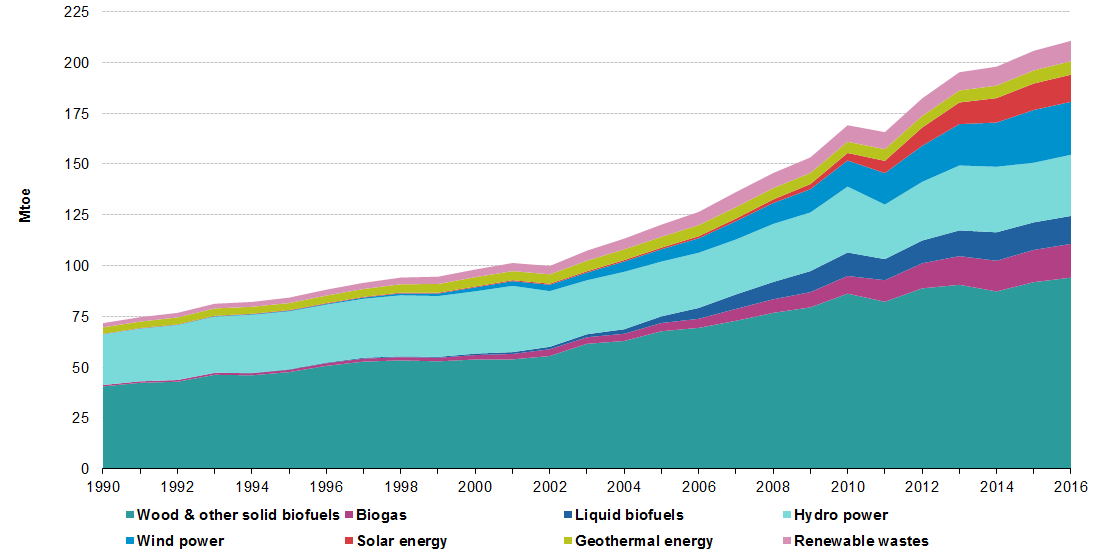
\includegraphics[width = \linewidth]{Images/Intro/Primary_production_of_energy_1990-2016.png}
		\caption{Production d'énergie primaire à partir de sources renouvelables en Europe de 1990 à 2016 d'après les chiffres d'Eurostat}
		\label{fig:Intro_EnergyProduction}
	\end{center}
\end{figure}

Cette intégration croissante des énergies renouvelables à production incertaine demande d'être faite avec minutie car elle impose de nouvelles formes d'incertitudes. %Cependant, elles peuvent aussi être vectrice de nouvelles opportunités.

Afin de comprendre pourquoi, il est nécessaire de faire un point sur le réseau électrique Français, et par extension, Européen. Ces réseaux se sont construits autour de l'impératif d'être en mesure de fournir, à n'importe quel instant, la puissance demandée par les utilisateurs. Or comme l'énergie qui circule sur les réseaux électriques est un flux instantané, une contrainte physique impose que demande et production soient égales à tout instant.

Les sources de productions d'énergies d'alors étaient principalement délocalisées, constantes et avec une faible inertie (centrales thermiques) ou forte inertie (centrale nucléaires).  Contraintes auxquelles il faut ajouter la difficulté de stockage de l'électricité ainsi que des infrastructures qui limitent la puissance de certains échanges. Pour pallier à ces difficultés et contraintes, plusieurs systèmes correspondant à différentes échelles de temps ont été mis en place.

%L'égalisation de la production et de la consommation aux temps long est peut être celle qui a été la moins problématique à l'heure actuelle. Il \textit{suffit} de s'assurer que les infrastructures en places et futures garantiront une production suffisante pour combler l'évolution de la demande. Les matières premières et énergies fossiles étant encore largement présente, beaucoup d'options de production d'énergies à moyen terme restent disponibles.

L'essentiel de l'organisation pour égaliser production et consommation aux temps moyens et courts réside dans la mise en place de différents marchés. Un premier ,le marché \textit{day-ahead}, sur lequel des accords non engageants sont pris pour le lendemain basés sur les particularismes de la journée (vague de froid, jour férié,... etc). Un autre marché a lieu au cours de la journée où des offres sont effectuées dès qu'elles sont compatibles. Cependant des écarts plus ou moins grands par rapport aux engagements ont lieux. Le gestionnaire de réseau fait alors appel à un second marché plus onéreux, dit marché de \textit{balancing}, pour combler ces écarts. En fonction des législation, les écarts par rapports aux engagements sur les différents marchés peuvent être soumis à des pénalisations.

Dans ce contexte, de nombreuses études avaient été réalisées sur la prévision de la consommation des ménages qui était à l'époque la principale source d'incertitude. Avec l'arrivée des énergies renouvelables à production incertaine, un important effort de recherche à été orienté autour de la prévision de production. Dans le cas de l'éolien et du photovoltaïque, ces prévisions sont souvent basées sur des prévisions météorologiques.

Étudier les erreurs de prévisions prend son sens au travers de plusieurs éléments. Tout d'abord, le fait que les prévisions de production soient basées sur des prévisions météorologiques empêche un rafraîchissement continu des prévision. En effet, les calculs météorologiques étant particulièrement lourds, ils ne sont réalisés que quelques fois par jour. Déterminer une dynamique dans les erreurs de prévisions permettrait donc d'affiner les prévisions de production entre deux mises à jour successives des calculs météorologiques. Enfin, au vu de la conception des marchés, ce sont bien les erreurs de prévisions qui doivent être compensés sur le second marché et qui peuvent perturber le réseau côté gestionnaire ou donner lieu à des amendes côté producteur. C'est donc bien, in fine, cette valeur qu'il est impératif de minimiser. Caractériser les erreurs de prévision est donc une approche complémentaire et une seconde source d'information valable et pertinente.  



\chapter{Présentation des données}
\section{Production Éolienne}
%\subsection{Données de Californie (BPA)}
L'étude est réalisée dans un premier temps sur des données issue de \href{https://transmission.bpa.gov/Business/Operations/Wind/}{Bonneville Power Administration} \footnote{\url{https://transmission.bpa.gov/Business/Operations/Wind/}} entre 2009 et 2017. Ces données comportent, par pas de temps de 5 minutes, les productions électriques éoliennes réelles ainsi que les prévisions à 1 heure annoncées par les producteurs.

Afin de réduire la taille du jeu de données, il est réduit à un échantillonnage horaire. Pour ce faire la moyenne sur l'heure suivante est réalisée.

D'autre part, comme le nombre d'installations de production à évoluée du simple au double (voir \href{https://transmission.bpa.gov/business/operations/Wind/WIND_InstalledCapacity_Plot.pdf}{ici} \footnote{\url{https://transmission.bpa.gov/business/operations/Wind/WIND_InstalledCapacity_Plot.pdf}}) sur cette période, les données ont été normalisées par la capacité de production maximale (voir \ref{fig::PredErrors_all}). Les erreurs de prévisions sont donc reconstituées à partir de ces données en soustrayant les productions mesurées aux productions prévues (voir \ref{fig:Data_BPA_WholeNorm}).


\begin{figure}[ht!]
\begin{center}
\begin{subfigure}[b]{0.45\textwidth}
	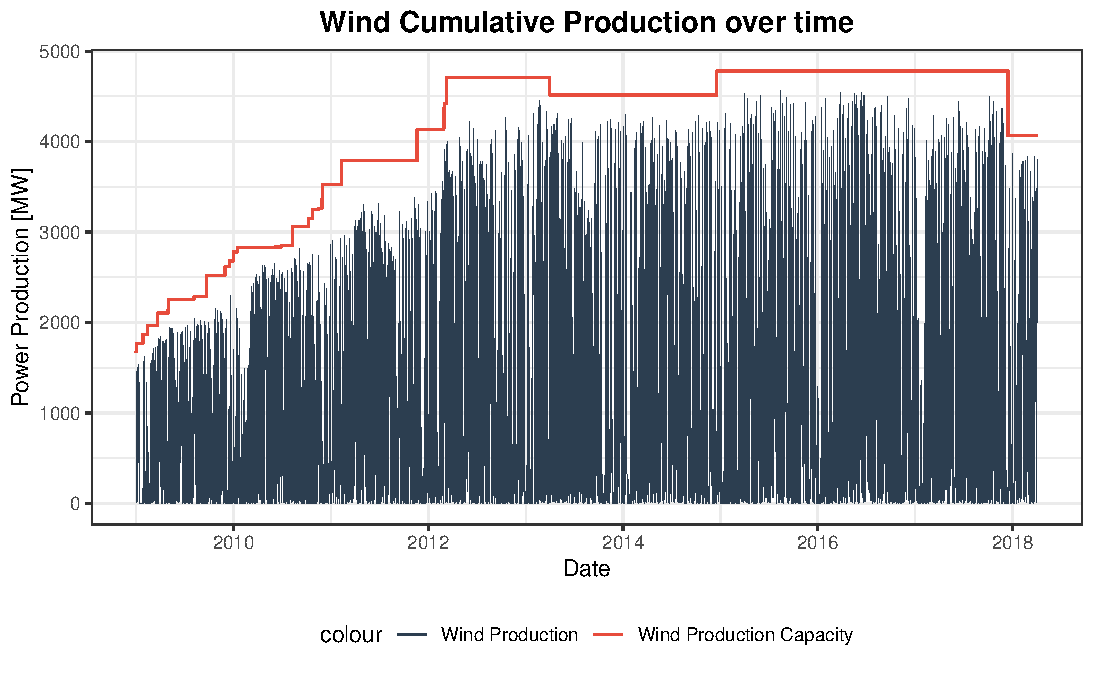
\includegraphics[width=\textwidth]{Images/Data/Eolien/BPA/Normalize.pdf}
	\caption{Production réalisée et capacité de production installée}
	\label{fig::PredErrors_all}
\end{subfigure}
~
\begin{subfigure}[b]{0.45\textwidth}
	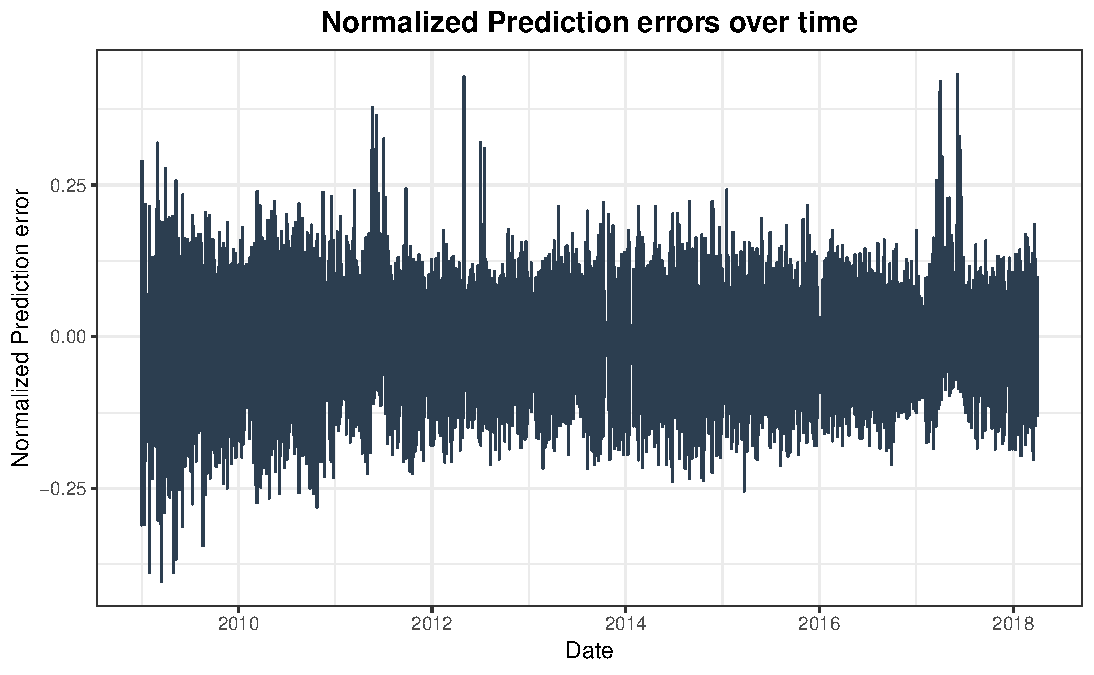
\includegraphics[width=\textwidth]{Images/Data/Eolien/BPA/NormWindErrs_All.pdf}
	\caption{Erreurs de prévisions normalisées }
	\label{fig:Data_BPA_WholeNorm}
\end{subfigure}
\caption{Représentation du jeu de donnée utilisé pour l'étude sur la période  allant de Janvier 2009 jusqu'à Mai 2018 }
\label{fig::DataPres}	
\end{center}
\end{figure}

La figure \ref{fig::Data_Eolien_BPA_HistNormERR} présente l'histogramme des erreurs normalisées en échelle logarithmique. On constate que les erreurs sont bien centrées autour de zéro et qu'une grande partie réside dans l'intervalle $[-0.2,0.2]$ \todo{Préciser combien} ce qui témoigne d'une relativement bonne capacité de prévision.
La figure \ref{fig::Data_Eolien_BPA_NormWindErrs_1Month} représente quand à elle un zoom sur la série temporelle des erreurs de prévisions. Il est intéressant de noter que la série présente des période sur lesquelles la variance est relativement faible (comme autour du 3 ou après le 8 décembre) et d'autre ou la variance est nettement plus élevée (comme sur la deuxième partie du mois).

\begin{figure}[ht!]
	\begin{center}
		\begin{subfigure}[b]{0.45\textwidth}
			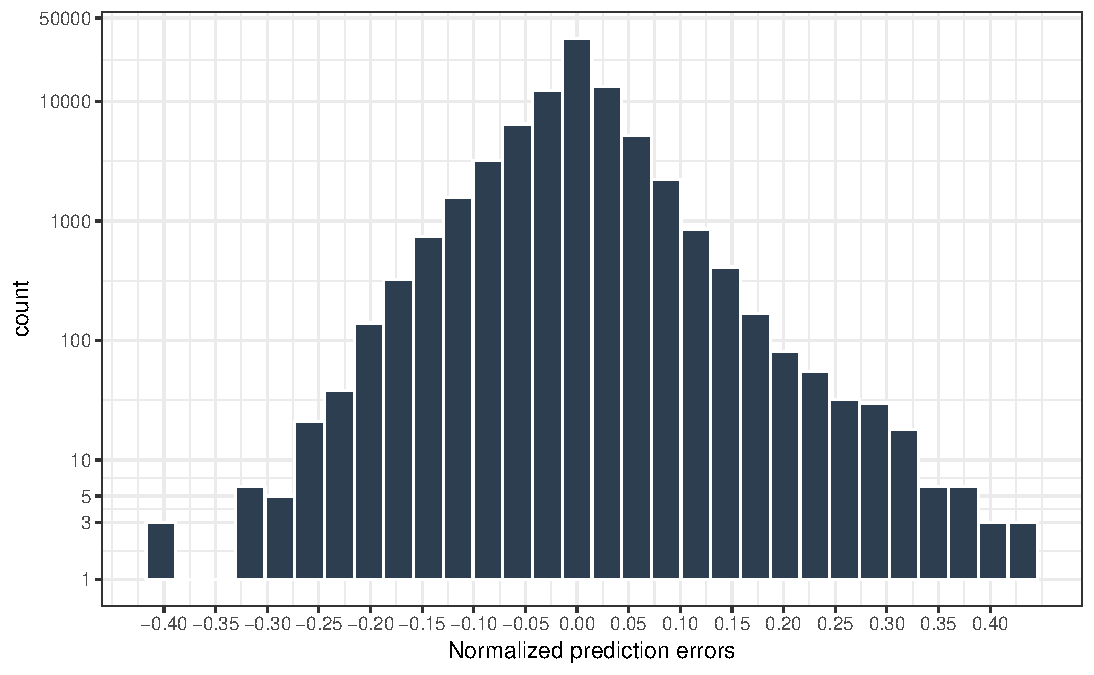
\includegraphics[width=\textwidth]{Images/Data/Eolien/BPA/Hist_NormErr.pdf}
			\caption{Histogramme des erreurs de prévisions}
			\label{fig::Data_Eolien_BPA_HistNormERR}
		\end{subfigure}
		~
		\begin{subfigure}[b]{0.45\textwidth}
			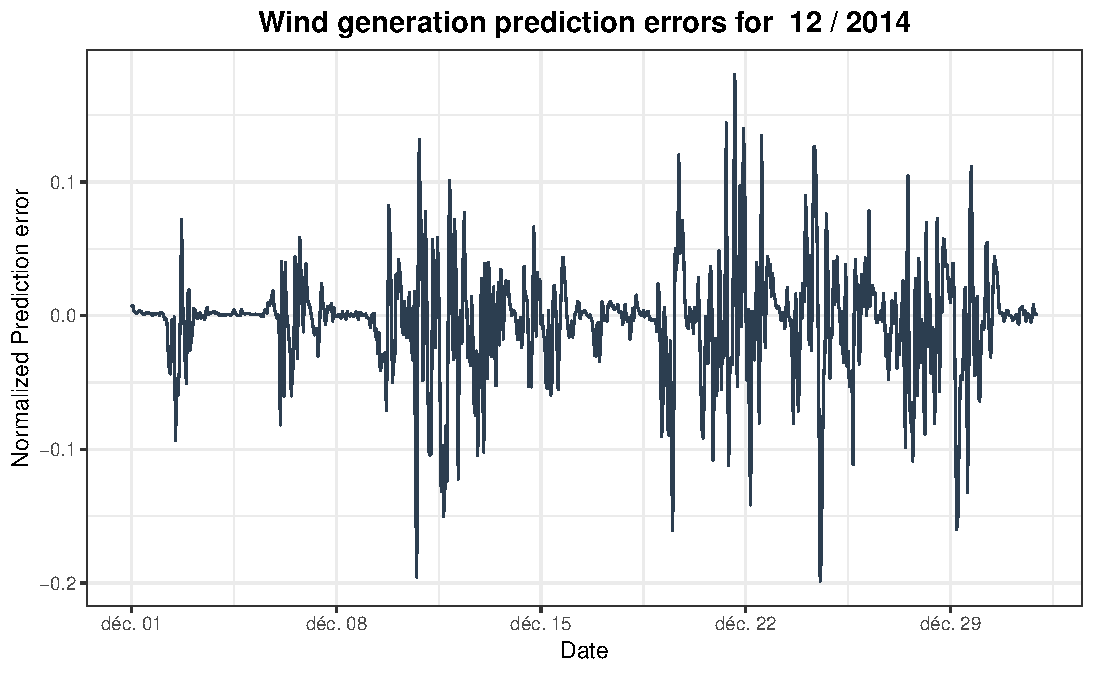
\includegraphics[width=\textwidth]{Images/Data/Eolien/BPA/NormWindErrs_1Month.pdf}
			\caption{Erreurs de prévisions sur un mois}
			\label{fig::Data_Eolien_BPA_NormWindErrs_1Month}
		\end{subfigure}
		\caption{Représentation du jeu de donnée utilisé pour l'étude}
		\label{fig::Data_BPA_HitsZoom}	
	\end{center}
\end{figure}

\section{Production Photovoltaïques}
%\subsection{Données Bavière (TenneT)}
Des données agrégées de production d'énergie photovoltaïque ainsi que les prévisions $J-1$ correspondantes sont mises à disposition par TenneT sur leur \href{https://www.tennet.eu/electricity-market/transparency-pages/transparency-germany/}{site web} \footnote{\url{https://www.tennet.eu/electricity-market/transparency-pages/transparency-germany/}}. Les données fournies sur la Bavière ont été utilisées pour cette étude. Ces données sont libres d'accès et ouvertes à la publication scientifique. Elles vont du $1^{er}$ décembre 2010 jusqu'à aujourd'hui avec un pas d'échantillonnage de 15 minutes (voir figure \ref{fig::Donnees_TenneT_Bayern_WHole}). Aucune covariable n'est mise à disposition. N'ayant pas eu accès à la capacité de production installée en Bavière sur cette période, ces données sont normalisées par des maxima de prévisions/productions sur certaines périodes. Cette capacité de production installée estimée est aussi représentée sur la figure \ref{fig::Donnees_TenneT_Bayern_WHole}. Les données manquantes (190 pour les prévisions et 69 pour les réalisations) sont remplacées par la dernière valeur observée temporellement parlant. 

\begin{figure}[ht!]
	\begin{center}
		
		\begin{subfigure}[b]{0.45\textwidth}
			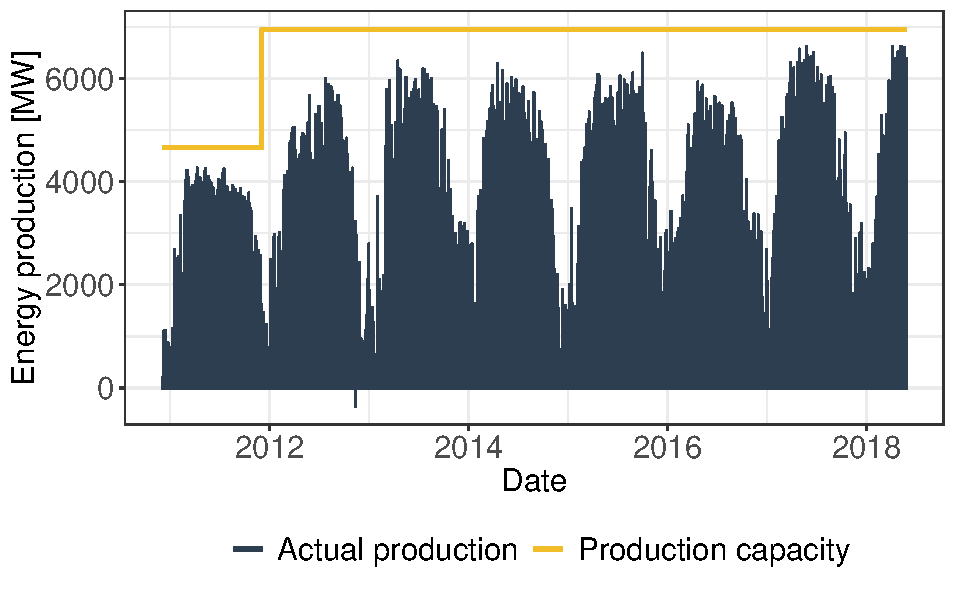
\includegraphics[width=\textwidth]{Images/Data/PV/Tennet/Tennet_Actual.pdf}
		\end{subfigure}
		~
		\begin{subfigure}[b]{0.45\textwidth}
			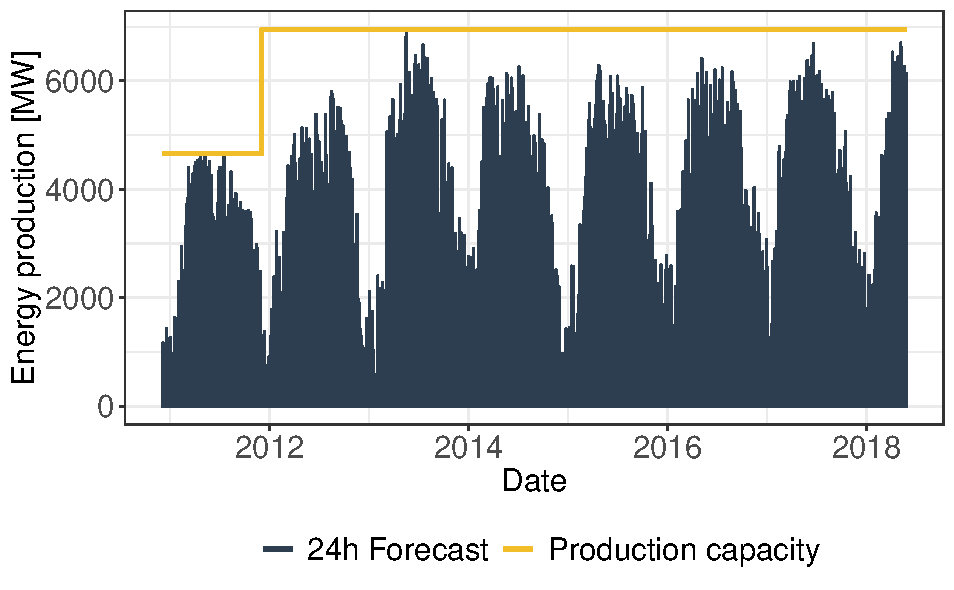
\includegraphics[width=\textwidth]{Images/Data/PV/Tennet/Tennet_Forecast.pdf}
		\end{subfigure}
		
		\caption{Production réelle (à gauche)  et prévue (à droite) d'énergie photovoltaïque en Bavière entre 2010 et aujourd'hui}
		\label{fig::Donnees_TenneT_Bayern_WHole}
		
	\end{center}
\end{figure}

La série temporelle des erreurs de prévisions alors obtenue est présentée sur la figure \ref{fig:Data_PV_PredErrs}. Comme l'illustre la partie zoomée, la structure de ces données est particulière avec une alternance de plages a valeurs négligeables et non négligeables.

\begin{figure}	
	\begin{center}
		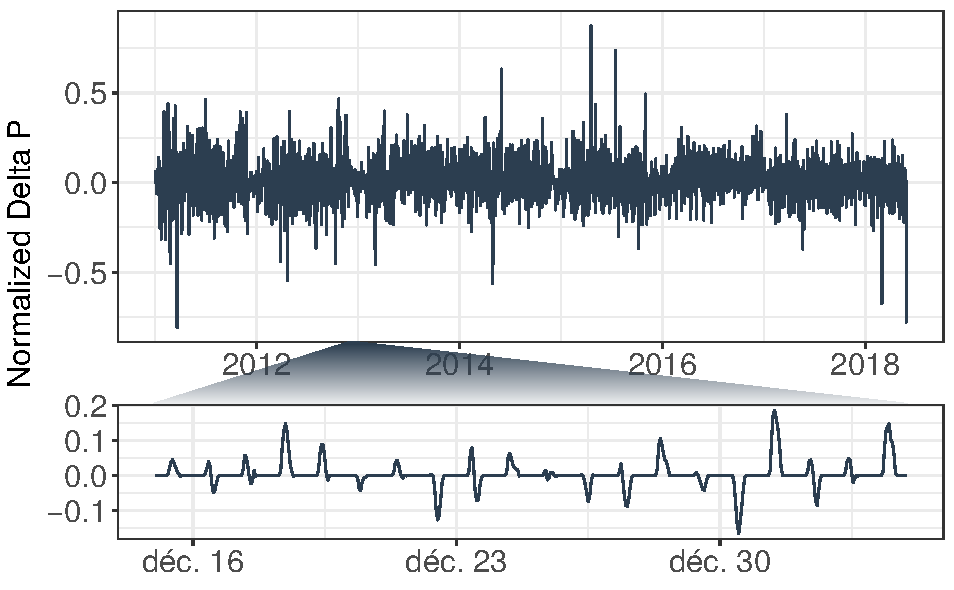
\includegraphics[width = 0.8 \textwidth]{Images/Data/PV/Tennet/TennetPrdErrors_WholeZoom_Mod.pdf}
		\caption{Erreur de prévision de production d'énergie solaire sur la Bavière}
		\label{fig:Data_PV_PredErrs}
	\end{center}
\end{figure}

Cette structure correspond en fait à une saisonnalité quotidienne comme le montre le diagramme en boîte de la figure \ref{fig:Data_TenneT_Bayern_BoxHist}. Les erreurs de prévisions entre 20h et 4h du matin sont systématiquement nulles. Elles correspondent aux plages horaires pendant lesquelles le soleil ne brille jamais en Bavière. En effet, à Munich (capitale de la Bavière), le soleil s'est levé à 5h12 et s'est couché à 21h17 le 21 Juin 2018. Sur ces périodes, aucune production d'énergie n'est prévue ni réalisée, et donc les erreurs sont systématiquement nulles.  Il est donc logique que les erreurs moyennes jusqu'à 5h du matin soient nulles. Cependant, au vu de cette amplitude d'ensoleillement maximale, il est possible qu'un autre phénomène réduise systématiquement les erreurs de prédiction a 20h et 21h pour lesquelles cette analyse n'explique pas d'aussi faible valeurs. L'histogramme aussi présenté sur cette figure illustre aussi cette surreprésentation des valeurs très faible. D'autre part, il montre que la grande majorité des erreurs de prévisions moyennées sont assez faibles. Par exemple, $90 \%$ des données sont incluses dans l'intervalle $[-0.688 , 0.0891]$. 

\begin{figure}[ht!]
	\begin{center}
		
		\begin{subfigure}[b]{0.45\textwidth}
			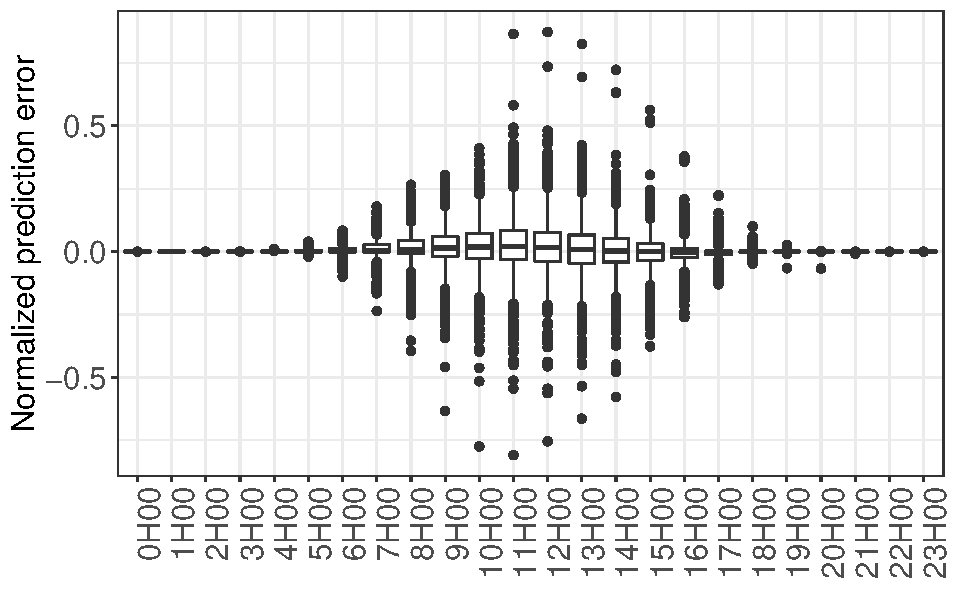
\includegraphics[width=\textwidth]{Images/Data/PV/Tennet/TennetBayern_Boxplot.pdf}
		\end{subfigure}
		~
		\begin{subfigure}[b]{0.45\textwidth}
			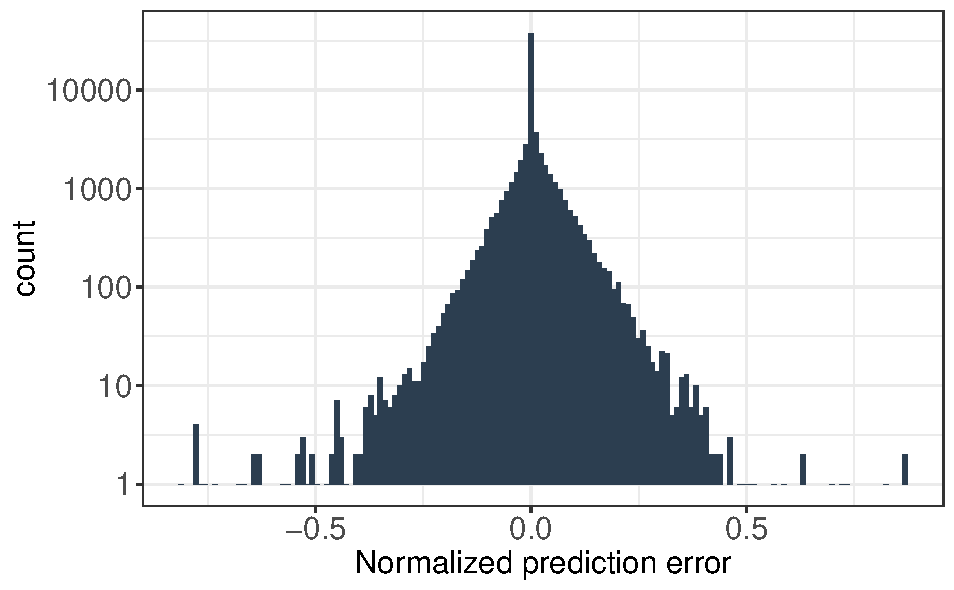
\includegraphics[width=\textwidth]{Images/Data/PV/Tennet/Data_Tennet_Histogram.pdf}
		\end{subfigure}
		
		\caption{Diagramme en boîte et histogramme pour les erreurs de prévisions moyennées sur chaque heure}
		\label{fig:Data_TenneT_Bayern_BoxHist}
		
	\end{center}
\end{figure}



\pagestyle{corpus}
\chapter{Modèles et métriques}

\section{Modèles de Markov cachés}
\nomenclature{HMM}{Modèle de Markov Caché ( \ref{subsec:Modeles_HMM} )}
\nomenclature{MS-AR}{Modèle Markov Switching Auto Regressive (\ref{subsec:Modeles_MSAR})}
\subsection{Chaîne de Markov}
Afin d'introduire correctement les modèles de Markov cachés il est d'abord nécessaire d'introduire le concept de chaîne de Markov. Les éléments constitutifs d'une chaîne de Markov sont :

\begin{tcolorbox}[colback=Blue_FlatUI!5,colframe=Blue_FlatUI,title=\textbf{Chaîne de Markov}]
	\begin{description}
		\item[$\bm{E}=\{ E_1,E_2,...,E_m\}$] Une liste de $m$ états possible 
		\item[$\bm{\Gamma$}] Matrice de probabilité de transition (de taille $m \times m$) d'un état à un autre. L'élément $(i,j)$, noté $\gamma_{ij}$, est la probabilité de transition de l'état $i$ à l'état $j$. Comme ce sont des probabilités alors 
		\begin{equation*}
		\sum\limits_{j=1}^m \gamma_{ij} = 1 \quad \forall i \in 1,2,...,m 
		\end{equation*}
		\item[$\bm{\pi}$=$\pi_1,\pi_2,...\pi_m$] où $\pi_i$ représente la probabilité initiale d'être dans l'état $i$.
	\end{description}
\end{tcolorbox}

\nomenclature{$m$}{Nombre d'états cachés (HMM et MSAR)}
\nomenclature{$\Gamma$}{Matrice de transition entre les états cachés (HMM et MSAR)}
\nomenclature{$\bm{\pi}$}{Probabilités initiales d'appartenance à l'un ou l'autre des états cachés (HMM et MSAR)}

Une séquence de variables discrètes $\{ C_t : t \in \mathbb{N} \}$ à valeurs dans $\bm{E}$ forme une chaîne de Markov si pour tout $t \in \mathbb{N}$ elle respecte l'hypothèse d'un processus Markovien \eqref{eq::HMM:MarkovProcess} :

\begin{equation}
P\left( C_{t+1} | C_t,C_{t-1},...,C_1  \right) = P\left( C_{t+1} | C_t  \right)
\label{eq::HMM:MarkovProcess}
\end{equation}

En d'autres terme, le processus n'a donc pas de mémoire et toute l'information utile pour prévoir l'état suivant est contenue dans l'état présent, comme le montre la figure \ref{fig::HMM:MarkovChain}.

D'autre part on introduit la terminologie suivante : si $P\left( C_{t+1} | C_t  \right)$ est indépendant de $t$ alors on parle de chaîne de Markov \textit{homogène}.

\begin{figure}[ht]
	\begin{center}
		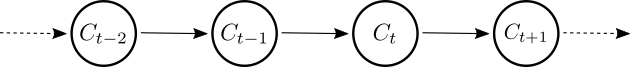
\includegraphics[width= 0.6 \textwidth]{Images/Models/HMM/ChaineMarkov.png}
		\caption{Représentation graphique d'une chaîne de Markov. Figure inspirée de \cite{zucchini_hidden_2017}.}
		\label{fig::HMM:MarkovChain}
	\end{center}
\end{figure}

\subsection{Modèle de Markov cachés}
\label{subsec:Modeles_HMM}
Une chaîne de Markov peut donc se révéler utile lors de la modélisation d'un phénomène observable. Cependant il arrive que le phénomène étudié ne soit que partiellement observable ou que l'on ne dispose pas de données pour le représenter. Un exemple didactique de l'utilité d'un HMM, imaginé par Jason Eisner, consistait en la détermination du caractère chaud ou froid de la journée en fonction du nombre de glaces mangées dans la journée. On a alors un processus caché à deux états (chaud ou froid) et une série d'observation (le nombre de glace mangées par jour). Un modèle de Markov caché est définit par les éléments suivants :

\begin{tcolorbox}[colback=Blue_FlatUI!5,colframe=Blue_FlatUI,title=\textbf{Modèlé de Markov caché  \hfill (HMM)}]
	\begin{description}
		\item[$\bm{E}=\{ E_1,E_2,...,E_m \}$] Une liste de $m$ états possible 
		\item[$\bm{\Gamma$}] Matrice de probabilité de transition (de taille $m \times m$) d'un état à un autre. L'élément $(i,j)$, noté $\gamma_{ij}$, est la probabilité de transition de l'état $i$ à l'état $j$. Comme ce sont des probabilités alors :
		\begin{equation*}
		\sum\limits_{j=1}^m \gamma_{ij} = 1 \quad \forall i \in 1,2,...,m 
		\end{equation*}
		\item[$\bm{X}=X_1,X_2,...,X_T$] Une séquence représentant le phénomène observé
		\item[$p_i(x)=P(X_t=x | E_i)  \quad \forall i =1,2,...,m$] La probabilité d'émission de l'observation $x$ sachant l'état $i$. Dans le cas d'observations continues, ceci peut être remplacé par une densité de probabilité.
		\item[$\bm{\pi}$=$\pi_1,\pi_2,...\pi_m$] où $\pi_i$ représente la probabilité initiale d'être dans l'état $i$.
	\end{description}
\end{tcolorbox}


L'idée fondamentale d'un modèle de Markov caché est de dire que l'observation ne dépend que de l'état dans lequel le système dynamique (la chaîne de Markov) se trouve. En considérant une séquence de $T$ variables discrètes $\bm{C}=C_1,C_2,...,C_T$ à valeurs dans $\bm{E}$ alors le système \eqref{eq::HMM:HmmEqns} est vérifié. Les hypothèses d'un modèle de Markov cachés sont représentées graphiquement dans la figure \ref{fig::HMM:HMM_Graph}. 

\begin{equation}
\begin{cases}
P\left( C_{t+1} | C_t,C_{t-1},...,C_1  \right) = P\left( C_{t+1} | C_t  \right)\\
P\left( X_t | \bm{X} , C_1,C_2,...,C_T \right) = P(X_t | C_t)
\end{cases}
\label{eq::HMM:HmmEqns}
\end{equation}

\begin{figure}[ht]
	\begin{center}
		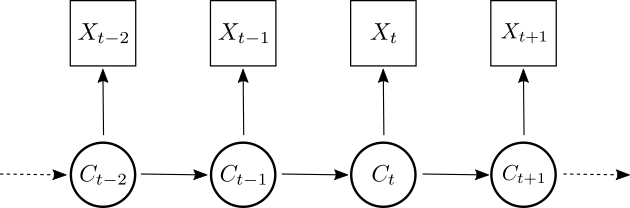
\includegraphics[width= 0.6 \textwidth]{Images/Models/HMM/HMM.png}
		\caption{Représentation graphique d'un modèle de Markov caché. Les flèches représentent les dépendances. Les carrés représentent les observations et les cercles le processus caché. Figure inspirée de \cite{zucchini_hidden_2017}.}
		\label{fig::HMM:HMM_Graph}
	\end{center}
\end{figure}

\nomenclature{$a_0$}{Moyenne des densités de probabilités (HMM) ou coefficient constant du processus auto-regréssif (MSAR)}
\nomenclature{$\sigma$}{Variance des densités de probabilités Gaussiennes de dimension $d \times d$ (HMM et MSAR)}
\nomenclature{$d$}{Dimension de l'espace}

Lors de ce stage, ce modèle a été utilisé pour caractériser des séries temporelles à variables continues et non discrètes. Les densités de probabilités utilisées ont à chaque fois été Gaussiennes et donc entièrement caractérisées par leurs moyennes $a_0$ et leurs variances $\sigma$. La complexité d'un tel modèle, dans le cas d'observations continues de dimension $d$, est donc la suivante :
\begin{equation}
\underbrace{m-1}_\text{Probabilités initiales}  + \underbrace{m \times d}_\text{Moyennes}  +  \underbrace{\frac{Kd \left(d - 1\right)}{2}}_\text{Matrices de variance covariance} + \underbrace{m \times m}_\text{Matrice de transition}
\label{eq:Model_HMM_ParamNumber} 
\end{equation}

Il a été montré précédemment dans \cite{rabiner_tutorial_1989} que les problèmes liés aux modèles de Markov cachés sont de trois natures différentes : 
\begin{itemize}
	\item Évaluation de la probabilité de l’observation d’une séquence.
	\item Recherche de la séquence le plus probable.
	\item Apprentissage
\end{itemize}

\subsubsection{Probabilité d’observation d’une séquence}
On se place dans  le cadre ou l'on dispose d'un HMM complet et on souhaite déterminer quelle est la probabilité d'obtenir une séquence d'observation précise. Plus formellement, en notant $\bm{X}$ la séquence observée et $\lambda$ le HMM considéré, on cherche $P(\bm{X}|\lambda)$.

En supposant que l'on connaisse la séquence d'états $\bm{C}$ alors il vient le résultat suivant :

\begin{equation}
P(\bm{X}|C_1,C_2,...,C_T) = \prod\limits_{i=1}^T P(X_i|C_i)
\end{equation}

Et comme cette séquence d'états $\bm{C}$ possède elle même une probabilité d'apparition, il vient :

\begin{equation}
P(\bm{X},\bm{C}) = P(\bm{X}|\bm{C}) \times P(\bm{C}) =   \prod\limits_{i=1}^T P(X_i|C_i) \times \prod \limits_{i=1}^T P(C_i|C_{i-1})
\end{equation}

Cependant, dans le cas des HMM, on ne connaît pas la succession d'états cachés qui a eu lieu pour générer cette séquence d'observation. Une méthode pour y remédier est de calculer la probabilité d'obtenir cette séquence par chaque combinaison de chemin. Traduit mathématiquement, cela donne :

\begin{equation}
P(\bm{X},\lambda) =\sum\limits_{\bm{C}} P(\bm{X}|\bm{C}) \times P(\bm{C}) 
\end{equation}

Le nombre total de séquences possibles dans le HMM $\lambda$ est de $m^T$. Dans un cadre réaliste, ou $T$ est grand et potentiellement $m$ aussi, ce calcul devient irréalisable. Pour y remédier, on utilise un algorithme progressif (communément appelé le forward algorithm) pour le calcul des probabilités. On introduit $\bm{P}(X)$ la matrice diagonale dont le $ii$-ième élément est $p_i(x)$ la probabilité d'obtenir l'observation $X$ depuis l'état $i$. On introduit de plus le vecteur $\bm{\alpha}_t$ dont la $j$-ième composante$ \alpha_t(j)$ est la probabilité d'être dans l'état $j$ après $t$ observations dans le cadre du HMM $\lambda$. Mathématiquement elle s'obtient de la façon suivante : 

\begin{equation}
\bm{\alpha}_t = \bm{\pi} \bm{P}(X_1) \times \prod\limits_{i=2}^t \bm{\Gamma}\bm{P}(X_i)
\end{equation}

On obtient donc l'algorithme récursif suivant dont le coût calculatoire n'est plus que de $T \times m^2$ :

\begin{align} 
\label{eq::HMM:ForwardAlgo}
\bm{\alpha}_1 &= \bm{\pi} \bm{P}(X_1) \\ 
\bm{\alpha}_t &= \bm{\alpha}_{t-1} \bm{\Gamma} \bm{P}(X_t)
\end{align}

\begin{figure}[ht]
	\begin{center}
		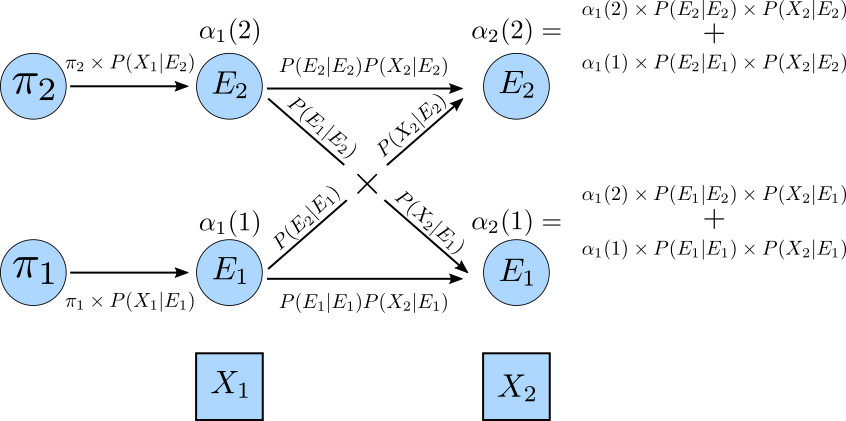
\includegraphics[width= 0.8 \textwidth]{Images/Models/HMM/Forward.png}
		\caption{Schéma du forward algorithm inspiré de \cite{jurafsky_speech_2017} }
		\label{fig::HMM:ForwardAlgo}
	\end{center}
\end{figure}

\subsubsection{Recherche de la séquence la plus probable}
On se place dans le cadre ou l'on dispose d'un HMM $\lambda$ et d'une série de $T$ observation $\bm{X}$. On cherche alors à déterminer quelle est la séquence d'états cachés $C_1,C_2,...,C_T$ qui a le plus de chance de générer cette séquence d'observation.

Encore une fois ce problème n'est pas viable en testant une à une les combinaisons afin de déterminer quelle est la plus probable. Pour y remédier, il est possible d'utiliser l'algorithme de Viterbi, dont la structure est assez similaire au forward algorithm. En effet il repose sur le même treillis mais la valeur en chaque maille représente la probabilité d'observer $X_t$ depuis l'état $C_i$ \textit{en ayant emprunté le chemin le plus probable menant à $C_i$}. A l'itération $t$ le vecteur de probabilités de Viterbi $\bm{v}_t$ se calcule donc de la manière suivante :

\begin{align} 
\label{eq::HMM:ViterbiAlgo}
\bm{v}_1 &= \bm{\pi} \bm{P}(X_1) \\ 
\bm{v}_t(j) &= \max\limits_{i=1}^m \left[ \bm{v}_{t-1}(i) \times \gamma_{ij} \times  p_j(X_t) \right] \quad \forall j \in 1,2,...,m
\end{align}

La séquence recherchée qui maximise la probabilité de réaliser l'observation est donc celle qui mène au $\max\left(\bm{v}_T\right)$. Lors du calcul, il est donc nécessaire de garder en mémoire le parcours effectué.

\begin{figure}[ht]
	\begin{center}
		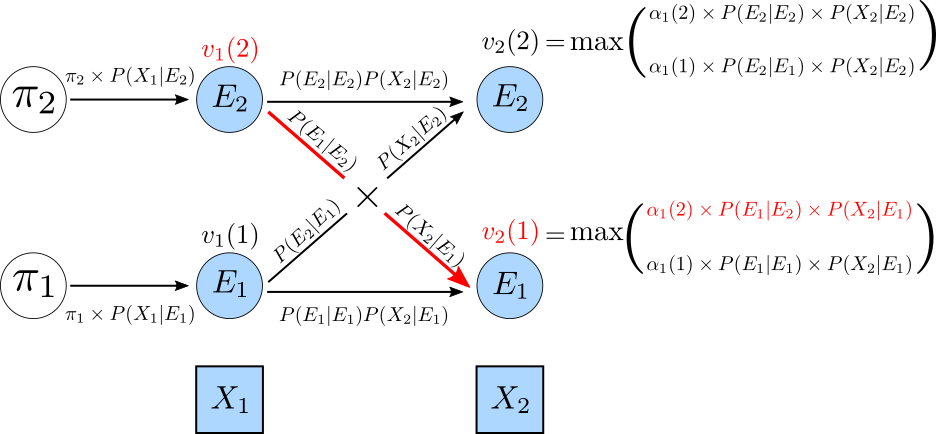
\includegraphics[width= 0.8 \textwidth]{Images/Models/HMM/Viterbi.png}
		\caption{Représentation du parcours du treillis par l'algorithme de Viterbi. Les cercles à fond blanc représentent les probabilités initiales ; les cercles à fond bleu les états et les carrés les observations. Les $v$ sont les probabilitées de Viterbi. Un maximum arbitraire à chaque $t$ est représenté en rouge pour illustrer le cheminement de la séquence la plus probable. Schéma inspiré de \cite{jurafsky_speech_2017}.}
		\label{fig::HMM:ViterbiAlgo}
	\end{center}
\end{figure}

\subsubsection{Apprentissage}
\label{subsubsec:Models_HMM_Apprentissage}
On se place dans le cadre ou l'on dispose d'une liste de $m$ états $\bm{E}$ et d'une séquence de $T$ observations $\bm{X}$. On cherche à déterminer la matrice de transition $\bm{\Gamma}$ et les probabilités d'émissions $p_i(x) \quad \forall i\in 1,2,...,m \quad \forall x \in \bm{X}$.

Pour ce faire il est possible de faire appel à un algorithme itératif nommé "forward backward". Celui-ci nécessite l'introduction d'une autre entité $\bm{\beta}_t$ qui est défini par l'équation \eqref{eq::HMM:BackwardProb}.

\begin{equation}
\bm{\beta}_t(i) = P(X_{t+1},X_{t+2},...,X_{T}|C_t=E_i)
\label{eq::HMM:BackwardProb}
\end{equation}

C'est un algorithme itératif qui calcule une estimation initiale des probabilités et qui utilise cette même estimation pour générer de meilleures probabilités. La première étape est de définir une formule pour calculer une estimation de $\gamma_{ij}$ que l'on notera $\hat{\gamma}_{ij}$ :

\begin{equation}
\hat{\gamma}_{ij} = \frac{\text{Nombre attendu de transitions entre } E_i \text{ et } E_j}{\text{Nombre total attendu de transitions depuis }E_i}
\end{equation}

En introduisant $\xi_t(i,j) = P(C_{t+1}=j,C_t=i|\bm{X},\lambda)$  On remarque que le numérateur pourrait alors s'écrire comme étant :

\begin{equation}
\sum\limits_{t=1}^{T-1} \xi_t(i,j) 
\end{equation}

D'autre part, on remarque qu'il est possible de calculer une quantité similaire à $\xi_t(i,j)$ :

\begin{equation}
\hat{\xi}_t(i,j) = P(C_{t+1}=j,C_t=i,\bm{X}|\lambda) = \alpha_t(i) \times \gamma_{ij} p_j(X_{t+1}) \times \beta_{t+1}(j)
\end{equation}

D'après l'identité $P(AB|C)=P(A|BC)P(B|C)$ on a :

\begin{equation}
\xi_t(i,j) = \frac{\hat{\xi}_t(i,j)}{P(\bm{X}|\lambda)} = \frac{\alpha_t(i) \times \gamma_{ij} p_j(X_{t+1}) \times \beta_{t+1}(j)}{\alpha_T(X_T)}
\end{equation}

Au final, on obtient :

\begin{equation}
\hat{\gamma}_{ij} = 
\frac{\sum\limits_{t=1}^{T-1} \frac{\alpha_t(i) \times \gamma_{ij} p_j(X_{t+1}) \times \beta_{t+1}(j)}
	{\alpha_T(X_T)}}
{\sum\limits_{k=1}^m \sum\limits_{t=1}^{T-1} \frac{\alpha_t(i) \times \gamma_{ik} p_k(X_{t+1}) \times \beta_{t+1}(k)}	   {\alpha_T(X_T)}}
\end{equation}

Il reste encore à déterminer les probabilités d'émissions. Pour cela on dérive une formule pour l'estimation de $p_i(x)$ : 

\begin{equation}
\hat{p}_i(X) = \frac{\text{Nombre attendu d'observations de }X\text{ depuis }i}
{\text{Nombre attendu d'occurrences  de }i}
\end{equation}

On introduit :

\begin{equation}
\kappa_t(j) = P(C_t=E_j|\bm{X},\lambda) = \frac{P(C_t=E_j,\bm{X}|\lambda)}{P(\bm{X}|\lambda)}
\end{equation} 

On est dans un cas particulier de la situation précédente avec $i=j$ et on obtient donc le résultat suivant :

\begin{equation}
\kappa_t(j) = \frac{\alpha_t(j)\beta_t(j)}{\alpha_T(X_T)}
\end{equation}

Au final :

\begin{equation}
\hat{p}_i(X) = \frac
{\sum\limits_{t=1}^T  \delta \kappa_t(i)}
{\sum\limits_{t=1}^T  \kappa_t(i)}
\quad \text{avec } \delta=
\begin{cases}
1\text{ si }X_t=X \\
0\text{ sinon}
\end{cases}
\end{equation}

Il est maintenant possible de raffiner l'estimation précédente de $\Gamma$ et des $p_i(x)$ à chaque itération. Cependant cet algorithme converge vers un minimum local. Il peut dont être important de déterminer une "bonne" estimation initiale.

\subsection{Modèles Markov Switching Auto-Regressive}
\label{subsec:Modeles_MSAR}
D'après le schéma \ref{fig::HMM:HMM_Graph}, l'utilisation d'un HMM pour représenter l'évolution d'une variable météorologique suppose que toute la dynamique est représentée par l'état caché. Or, notamment dans le contexte météorologique, il est clair que la probabilité d'une observation dépend de l'observation précédente. Pour affaiblir cette hypothèse il est possible d'utiliser des modèles de type MSAR où la dynamique de la série temporelle est décrite par une collection de modèles auto-régressifs. Le choix du modèle auto-régressif est alors contrôlé par une chaîne de Markov cachée. Le schéma \ref{fig::HMM:MSAR} représente graphiquement les dépendances d'un MSAR.

\begin{figure}[ht]
	\begin{center}
		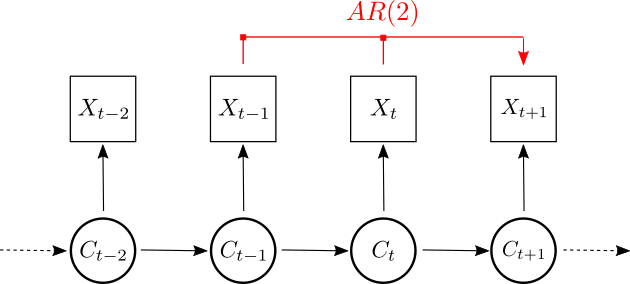
\includegraphics[width=0.6 \textwidth]{Images/Models/HMM/MSAR.png}
		\caption{Représentation des dépendances d'un modèle de type MSAR avec des modèles auto-régressifs d'ordre 2. Ici l'observation $X_{t+1}$ est générée à partir du modèle pointé par l'état caché $C_{t+1}$ qui prend en entrée les observations $X_t$ et $X_{t-1}$.}
		\label{fig::HMM:MSAR}
	\end{center}
\end{figure}


D'autre part, le fonctionnement des HMM à été présenté dans la section précédente pour des phénomènes à valeurs discrètes. Or les séries temporelles étudiées dans ce rapport sont continues. C'est pourquoi il convient de remplacer les probabilités d'émettre une observation spécifique $p_i(x)$ par les éléments constitutifs d'une densité de probabilité.


\section{Modèles GARCH}
Les modèles \textit{Auto-Regressive Conditionnal Heteroskedasticity} (ARCH) ont été introduit pour prendre en compte le caractère variable de la variance d'une série temporelle. ils se basent sur l'étude des résidus d'un processus modélisant la moyenne (ARIMA par exemple), notés $\epsilon_t$. Ces résidus ne doivent plus être auto-corrélés. Le modèle sépare alors ces résidus en deux parties distinctes avec $\sigma_t$ un écart type qui dépend du temps et $z_t$ une partie stochastique (un bruit blanc).

\begin{equation}
\epsilon_t = \sigma_t  z_t
\end{equation}

Le modèle ARCH modélise l'écart type de la façon suivante :

\begin{equation}
\sigma_t^2 = \alpha_0 + \alpha_1  \epsilon_{t-1}^2 + \alpha_2  \epsilon_{t-2}^2 + ... + \alpha_p  \epsilon_{t-p}^2 
\label{ARCH}
\end{equation}

Avec comme conditions que $\alpha_0 > 0$ et $\alpha_i \geq 0 \quad \forall \text{ } i \in [1,...,n] $. Une structure plus générale, le modèle \textit{Generalized ARCH} (GARCH), propose que l’écart type soit modélisé de la façon suivante :

$ \sigma_t^2 = \alpha_0 + \alpha_1  \epsilon_{t-1}^2 + ... + \alpha_p  \epsilon_{t-p}^2
+ \beta_{t-1} \sigma^2_{t-1} + ... + \beta_{t-q} \sigma^2_{t-q}$

\section{K-moyennes (Kmeans)}
\label{sec:Kmeans}
\nomenclature{Kmeans}{Méthode de partitionnement K-moyennes}

Le modèle des K moyennes est un est un modèle de partitionnement de données (ou souvent dit de \textit{"clustering"} d'après la dénomination anglaise). Le problème consiste donc à diviser un ensemble de points en un certains nombre de groupe $m$ de façon à ce qu'ils minimisent une certaine fonction.

Dans le cas présent, j'ai fait appel à la routine R \texttt{Kmeans}, qui cherche à minimiser la somme des erreurs quadratiques au sein de chaque groupe grâce à l'algorithme heuristique décrit dans \cite{hartigan_algorithm_1979}. Il fonctionne de la façon suivante : soit une partition de l'ensemble des points $C$. Alors, un point aléatoire $x$ est choisi et le centre du cluster auquel il appartenait est mis à jour comme si ce point ne lui appartenait plus. Le point choisi aléatoirement est ensuite réassigné au cluster qui permet de minimiser le plus possible la fonction de coût total, c'est à dire la somme des erreurs quadratiques au sein des clusters. Par construction, cet algorithme permet de ne jamais accroître la fonction de coût. Ainsi, il donne assurance qu'une partition dont les points sont fixés sera atteinte après un nombre fini d'itérations.

\section{Modèle de mélange gaussien (GMM)}
\nomenclature{GMM}{Modèle de mélange gaussien}
\label{sec:Model_GMM}
Le modèle de mélange de mélange gaussien est un modèle statistique qui tente d'expliquer une une distribution statistique comme étant une somme de sous distributions gaussiennes. La figure \ref{fig:GMM_ToyEx} présente un cas d'application idéaliste d'un tel modèle. 

\todo{Changer ou supprimer la figure}

\begin{figure}[ht]
\centering
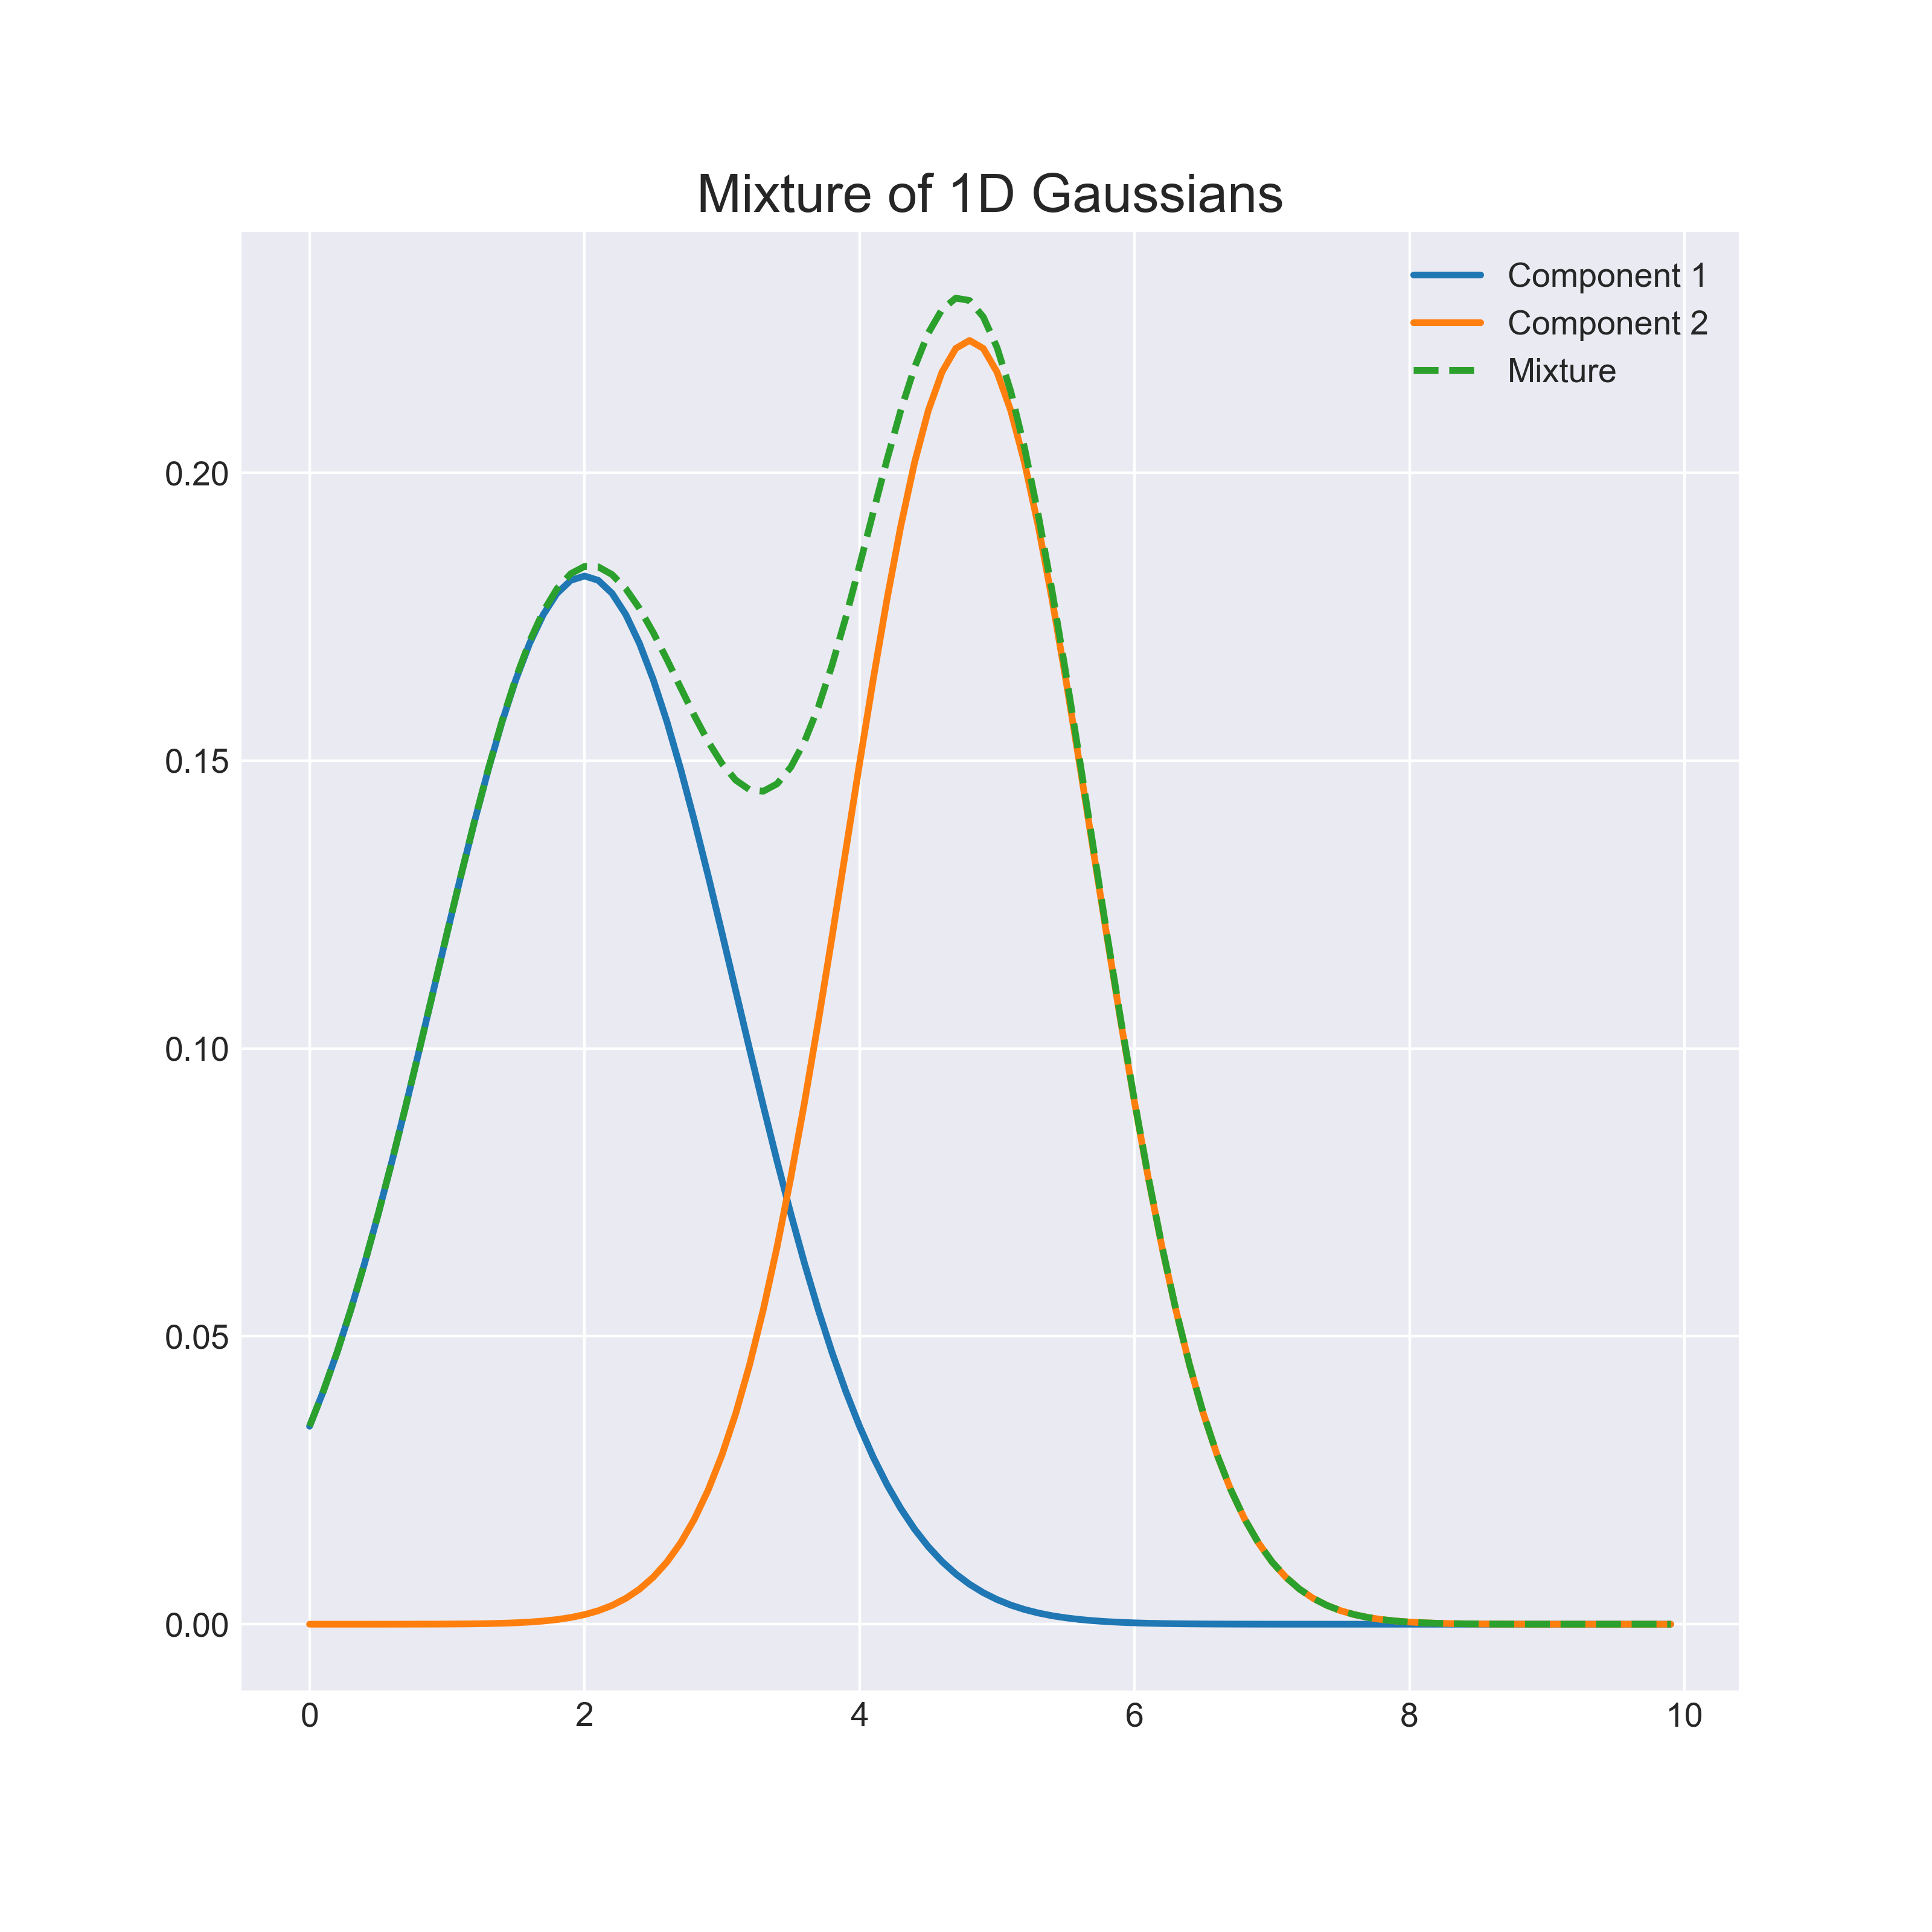
\includegraphics[width=0.5\linewidth]{Images/Models/GMM/GMM_toyexemple}
\caption{Exemple d'application d'un GMM dans un cas idéaliste }
\label{fig:fig:GMM_ToyEx}
\end{figure}



Ce modèle cherche donc à identifier, pour chaque gaussienne, sa variance, sa moyenne et les proportions. La gestion des problèmes en haute dimension avec ce modèle peut s'avérer difficile car il est sujet à la malédiction de la dimension. En effet, si $d$ est la dimension de l'espace et $m$ le nombre de clusters, alors le nombre de paramètres à identifier est :

\begin{equation}
	\underbrace{m-1}_\text{Proportions}  + \underbrace{m \times d}_\text{Centres}  +  \underbrace{\frac{md \left(d - 1\right)}{2}}_\text{Matrices de variance covariance}
	\label{eq:Model_GMM_ParamNumber} 
\end{equation}

On a donc le nombre de paramètres qui évolue de façon linéaire avec le nombre de clusters $m$ et quadratique avec la dimension $d$. Comme le montre \cite{bouveyron_model-based_2014}, il est préférable d'utiliser des modèles réduits ou par de la sélection de variable plutôt que de réduire l'espace dans lequel vivent les données. C'est pourquoi, au cours de ce stage, les paramètres des modèles de mélanges gaussiens ont été estimés via l'utilisation du package \texttt{Mclust}. En effet, il dispose d'une liste de modèles de mélange gaussien qui facilite la prise en compte de la haute dimension en réduisant le nombre de paramètres, comme explique dans \cite{scrucca_mclust_2016}. Il utilise, tout comme les modèles MS-AR, un algorithme EM pour identifier les jeux de paramètres maximisant la vraisemblance. 


\section{Analyse par Composante Principale}
\label{sec:Model_ACP}
\nomenclature{ACP}{Analyse par Composante Principale}

\section{Métriques}
\subsection{BIC}
\nomenclature{BIC}{Bayesian Information Criterion}
Le \textit{Bayesian Information Criterion}  permet de faire un compromis entre la vraisemblance des modèles vis-a-vis d'une série temporelle et leurs nombre de paramètres. Il est définit dans \eqref{eq:BIC} avec $L$ la vraisemblance, $k$ le nombre de paramètres du modèle et $N$ le nombre d'observations dans la série temporelle. Au vu de sa définition c'est un score orienté négativement. Le meilleur modèle au sens du critère BIC est donc celui qui obtiendra les valeurs les plus faibles.

\begin{equation}
BIC = - 2 \log L + k \log N
\label{eq:BIC}
\end{equation}

\subsection{Erreur moyenne absolue (MAE)}
\label{subsec:Model_Metric_MAE}
\nomenclature{MAE}{Erreur moyenne absolue}
L'erreur moyenne absolue est définie comme étant :
\begin{equation}
	MAE  = \frac{\sum_{i=1}^{T} \abs{\widetilde{P} - P} }{T}
	\label{eq:MAE}
\end{equation}

\subsection{Erreur quadratique moyenne (RMSE)}
\label{subsec:Model_Metric_RMSE}
\nomenclature{RMSE}{Erreur quadratique moyenne}
L'erreur quadratique moyenne est définie comme étant :

\begin{equation}
	RMSE = \sqrt{ \frac{\sum_{i=1}^{T} {\left( \widetilde{P} - P \right) } ^2 }{T}}
\end{equation}


\subsection{Erreur moyenne (BIAS)}
\nomenclature{BIAS}{Erreur moyenne}
\label{subsec:Model_Metric_BIAS}
%
%\subsection{Energy Score}
%On présente ici une métrique, l'Energy Score, qui cherche à qualifier la qualité d'un ensemble de scénarios générés dans un contexte de prédiction. Cette métrique est introduite dans \cite{tilmann_gneiting_probabilistic_2007} et son caractère discriminant a été discuté dans \cite{pinson_discrimination_2013}.Il pondère l'écart entre la réalité avec la moyenne des scénarios et la largeur du spectre des scénarios. En notant $J$ le nombre total de scénarios, $z_t$ la série réalisée et $\hat{z}_t^{j}$ le $j^{eme}$ scénario, l'\textit{Energy Score} est définit dans l'équation \ref{eq::EnergyScore}. C'est un score orienté négativement : le meilleur ensemble de scénarios obtiendra donc le score le plus faible.
%
%\begin{equation}
%ES = \frac{1}{J} \sum_{J=1}^{J} \norme{z_t - \hat{z}_t^{(j)}}_2 - \frac{1}{2J^2} \sum_{i=1}^{J} \sum_{j=1}^{J} \norme{\hat{z}_t^{(j)} - \hat{z}_t^{(j)}}_2
%\label{eq::EnergyScore}
%\end{equation}
 


\chapter{Erreurs de prévision éolienne}
\label{seq:ResultatsEolien}

L'application des modèles MS-AR aux erreurs de prévisions de production d'énergie éolienne a donné lieu à la rédaction d'une première version d'un article scientifique. Le lecteur est donc invité à lire ce document en annexe \ref{annex:ModelingWindPower}. Les travaux que j'ai effectués sont présentés dans la section intitulé \textit{Modelling of the wind power forecast error}. Les poursuites d'études, notamment celles concernant les transitions non homogènes, ont été commencées mais elles ne sont pas assez abouties pour être intégrées telles quelles dans ce rapport.

\chapter{Erreurs de prévision photovoltaïque}
Les erreurs de prédiction de production photovoltaïques diffèrent par nature de celles de production éolienne. Alors que le vent peut être d'intensité non négligeable à tout instant, l'irradiance sera quant à elle complètement nulle la nuit. Comme l'alternance jour/nuit est un phénomène purement déterministe les prévisionniste ne commettent pas d'erreurs de prévisions la nuit. Ceci modifie la structure des erreurs de prévisions en introduisant régulièrement des plages de prévisions nulles. Or les outils utilisés dans la section \ref{seq:ResultatsEolien} se heurtent à des problèmes de convergence numérique s'ils sont utilisés tels quels sur la série d'erreur de prédiction de production photovoltaïque. \todo{Expliquer pourquoi clairement}.

Afin de se ramener à une structure de série temporelle moins délicate en termes de résolution numérique, une approche simpliste aurait consisté à supprimer les périodes nocturnes de la série temporelle. Cependant, cette méthode fait part de deux désavantages qui à fait qu'elle a été écartée au cours de ce stage. Tout d'abord, même si elle paraît très simple, il faut malgré tout tenir compte que la durée de la nuit change tous les jours. De surcroît, cela imposerait un pré-traitement des données qui dépend aussi de leur origine géographique. Ainsi la méthodologie et le modèle obtenu paraît être trop difficilement transposable pour être un jour utilisé en opérationnel. C'est pourquoi une approche légèrement différente a été choisie.

En observant la série de donnée, il est possible de remarquer que des trajectoires quotidiennes typiques apparaissent. Cette approche à déjà été utilisée dans \cite{latimier_gestion_2016}, ce qui permet de se soustraire aux problèmes de convergences numériques en introduisant un autre difficulté : la haute dimension.

\section{Méthode des plus proches voisins}
Dans un premier temps, je me suis attaché à voir s'il était possible de corriger la prédiction fournie un jour à l'avance en fonction de l'allure des erreurs déjà observées dans la journée courante.

\nomenclature{$\widehat{d}$}{Indice de la journée indiquant l'heure de la correction}
On note $\widehat{d}$ l'indice de dimension indiquant quand la correction doit être réalisée. Alors nécessairement $\widehat{d} < d$. Pour le contexte applicatif, afin de se placer dans un cadre qui pourrait être réaliste au sens opérationnel, la correction doit être effectuer à 10h.

L'identification des journées les plus proches à été réalisé en sélectionnant celles qui minimisaient \eqref{eq:NN_identification} où $z$ représente la trajectoire de la journée courante et $\widetilde{z}$ une des trajectoires passées. 

\begin{equation}
	\sum_{i=1}^{\widehat{d}} \abs{z_i - \widetilde{z_i}}
	\label{eq:NN_identification}
\end{equation} 
 


La première étape dans l'utilisation de la méthode des plus proches voisins consiste à identifier quelle est le nombre optimal de plus proches voisins à prendre en compte. Dans cet objectif, il est nécessaire d'identifier une métrique pour évaluer le gain en terme  de prédiction. J'ai décidé d'utiliser comme critère \eqref{eq:KNN_identification} où $\overline{z_i^{NN}}$ représente la moyenne des plus proches voisins considérés.

\begin{equation}
	\frac{\sum_{i=\widehat{d}}^{d} \abs{z_i - \overline{z_i^{NN}} }}{\sum_{i=\widehat{d}}^{d} \abs{z_i}} 
	\label{eq:KNN_identification}
\end{equation}

La Figure \ref{fig:KNN_Intraday_scenarios} montre des exemples ou cette méthode de correction d'erreur fonctionne plus ou moins bien. Il est quand même intéressant de constater que même dans le cas où elle amplifierait l'erreur commise, plusieurs trajectoires parmi les voisins identifiés avaient capturées le bon comportement.

\begin{figure}[h] 
	\begin{subfigure}[b]{0.5\linewidth}
		\centering
		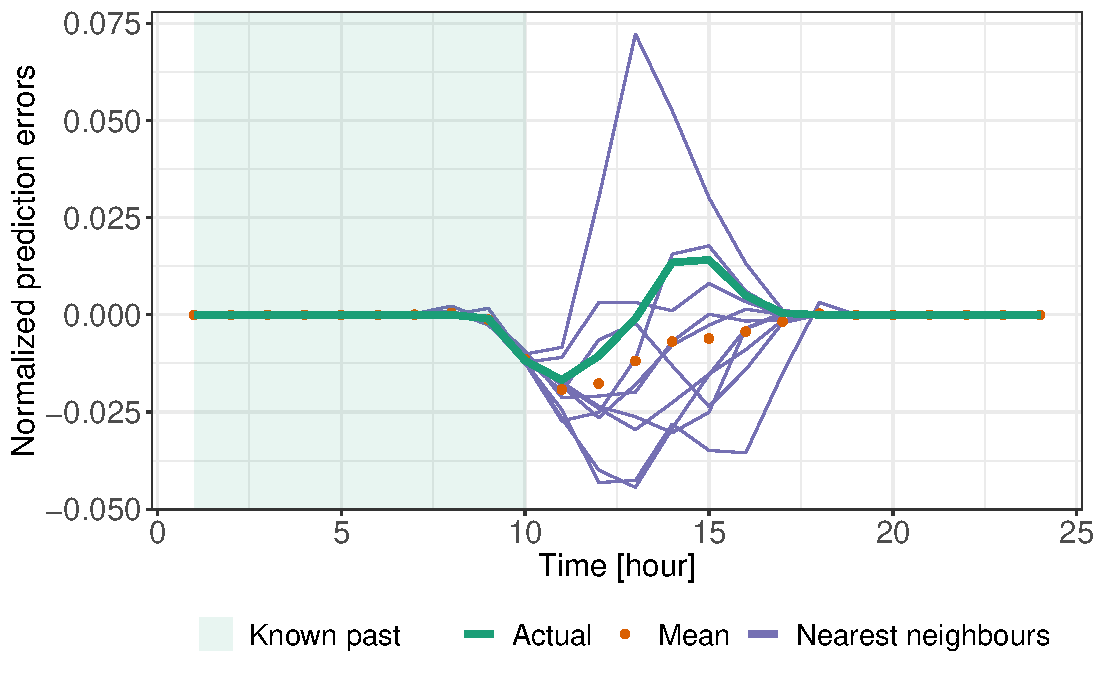
\includegraphics[width=1\linewidth]{Images/PV/KNN/NN_intraday_testdata_11.pdf} 
		%\caption{AR 1} 
		%\label{fig::HHMM_8HS_Traj_HS1} 
		%\vspace{4ex}
	\end{subfigure}%% 
	\begin{subfigure}[b]{0.5\linewidth}
		\centering
		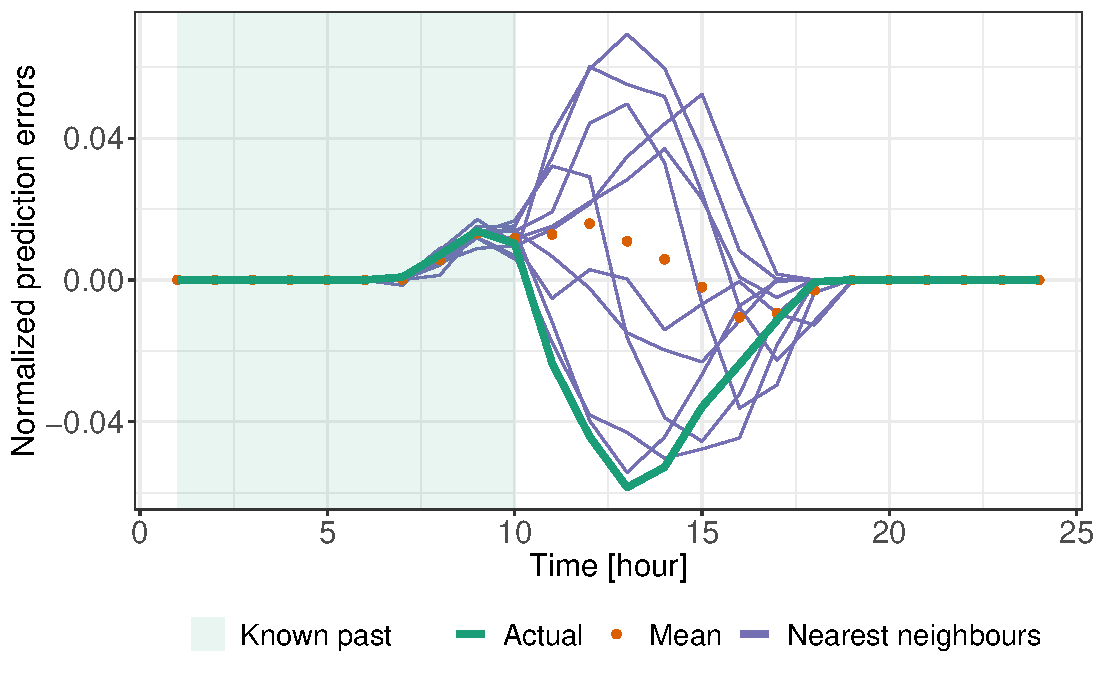
\includegraphics[width=1\linewidth]{Images/PV/KNN/NN_intraday_testdata_48.pdf} 
		%\caption{AR 2} 
		%\label{fig::HHMM_8HS_Traj_HS2} 
		%\vspace{4ex}
	\end{subfigure}
	\centering
	\begin{subfigure}[b]{0.5\linewidth}
		\centering
		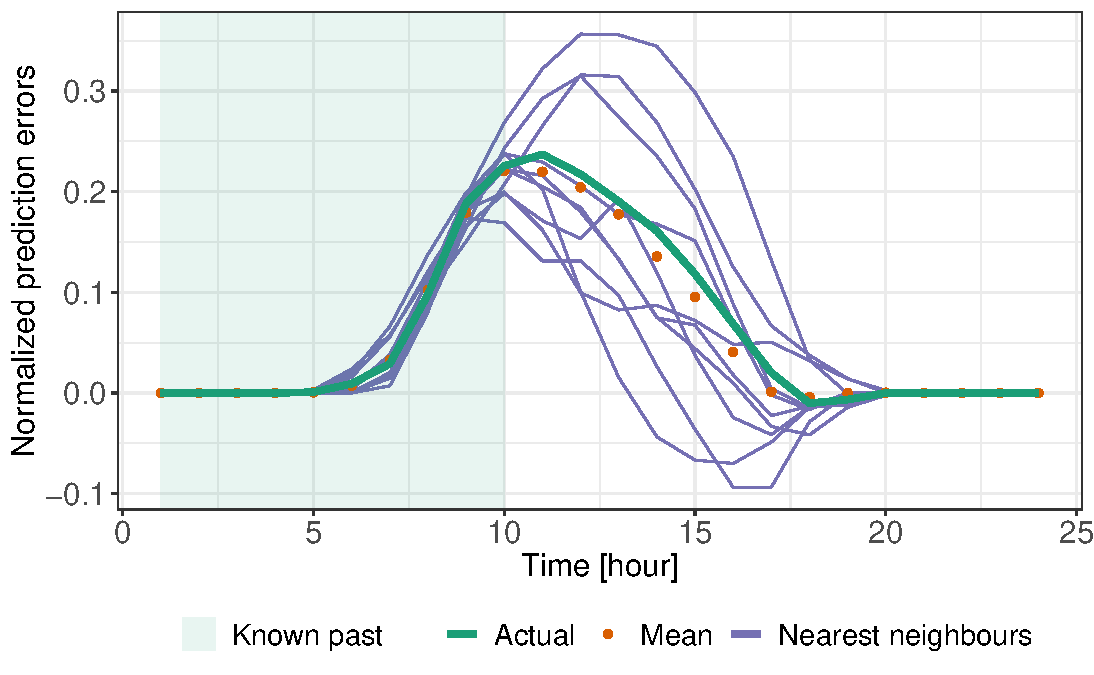
\includegraphics[width=1\linewidth]{Images/PV/KNN/NN_intraday_testdata_99.pdf} 
		%\caption{AR 3} 
		%\label{fig::HHMM_8HS_Traj_HS3} 
	\end{subfigure}%%
	
	\caption{Exemples de trajectoires d'erreurs de prévisions ainsi que les 10 trajectoires les plus proches identifiés via \eqref{eq:NN_identification} et leur moyenne}
	\label{fig:KNN_Intraday_scenarios} 
\end{figure}


La comparaison des performances en fonction du nombre de plus proches voisins est présentée dans la Figure \ref{fig:KNN_Comp}, avec le label \textit{all}. On remarque que, dans la limite des cas testés, l'augmentation du nombre de plus proches voisins ne dégrade pas les résultats obtenus. Cependant, en se limitant aux 5 premiers voisins on obtient une réduction de l'erreur sur le reste de la journée de l'ordre de $30\%$.

Cependant, comme cette méthode requiert d'identifier la trajectoire courante parmi toutes les trajectoires connues, elle peut s'avérer très coûteuse en temps de calcul au fil du temps. Par ailleurs, son comportement va par définition évoluer au cours du temps, ce qui peut amener à des déconvenues. Une option pour limiter cet effet négatif réside dans la détermination de trajectoires types. En effet, en regardant la figure \ref{fig:KNN_Intraday_scenarios}, on peut observer des trajectoires d'erreurs typique en forme de paraboles positive ou négative centrée autour de 14h. D'où l'idée d'identifier les plus proches voisins non plus parmi l'ensemble des trajectoires disponibles mais depuis des trajectoires représentatives.

L'identification de ces trajectoires à été réalisée grâce à la méthode des Kmeans (voir \ref{sec:Kmeans}). La figure \ref{fig:Kmeans_centers} présente les trajectoires types obtenues pour différents nombres de classes. Au vu du contexte, le nombre optimal de classe a été choisi en comparant les résultats obtenus pour de la correction d'erreur. Ces résultats sont présentés dans la figure \ref{fig:KNN_Comp}. Tout d'abord, l'identification des plus proches voisins parmi ces groupes détériore systématiquement les résultats par rapport à l'identification sur tout le passé connu. Cependant en identifiant la moyenne d'environ 5 trajectoires types parmi 20, une correction d'erreur de l'ordre de $25 \%$ peut être atteinte.

\begin{figure}[h]
	\centering
	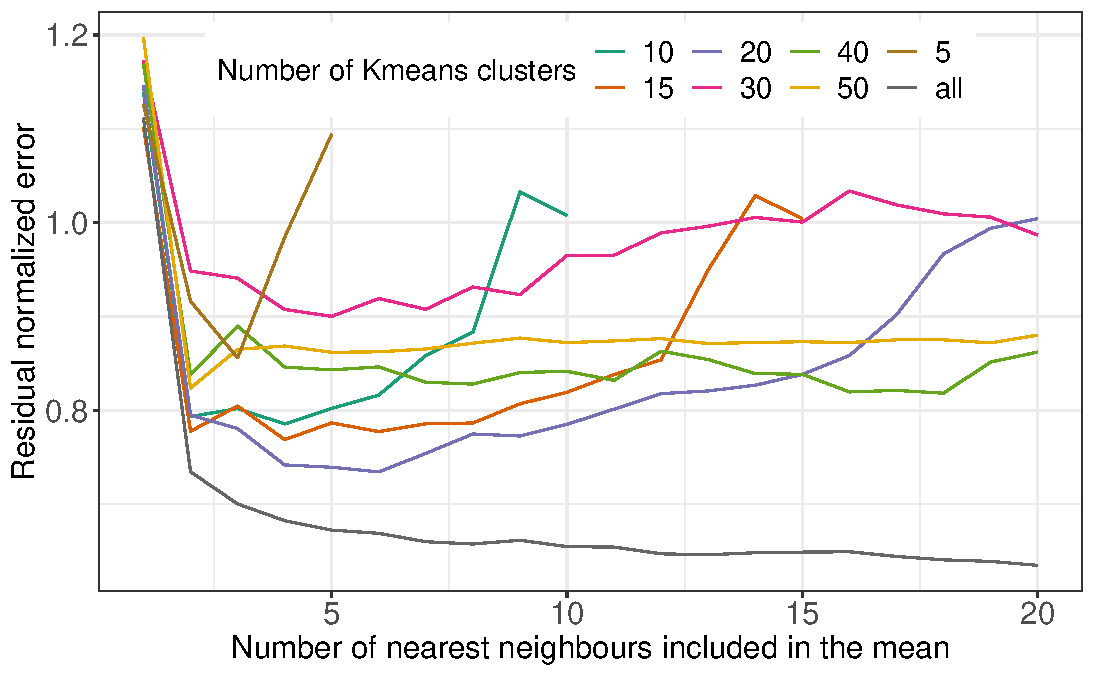
\includegraphics[width=0.75\linewidth]{Images/PV/KNN/KNN_compare.pdf}
	\caption{Comparaison des corrections de prévisions en fonction du nombre de plus proches voisins. La série \textit{all} présente les résultats quand les plus proches voisins sont identifiés parmi toutes les trajectoires du jeu de données d'entraînement. Les autres, quand ils sont identifiés parmi un certain de clusters obtenus par la méthode des Kmeans (voir section \ref{sec:Kmeans})}
	\label{fig:KNN_Comp}
\end{figure}

\begin{figure}[h] 
	\begin{subfigure}[b]{0.5\linewidth}
		\centering
		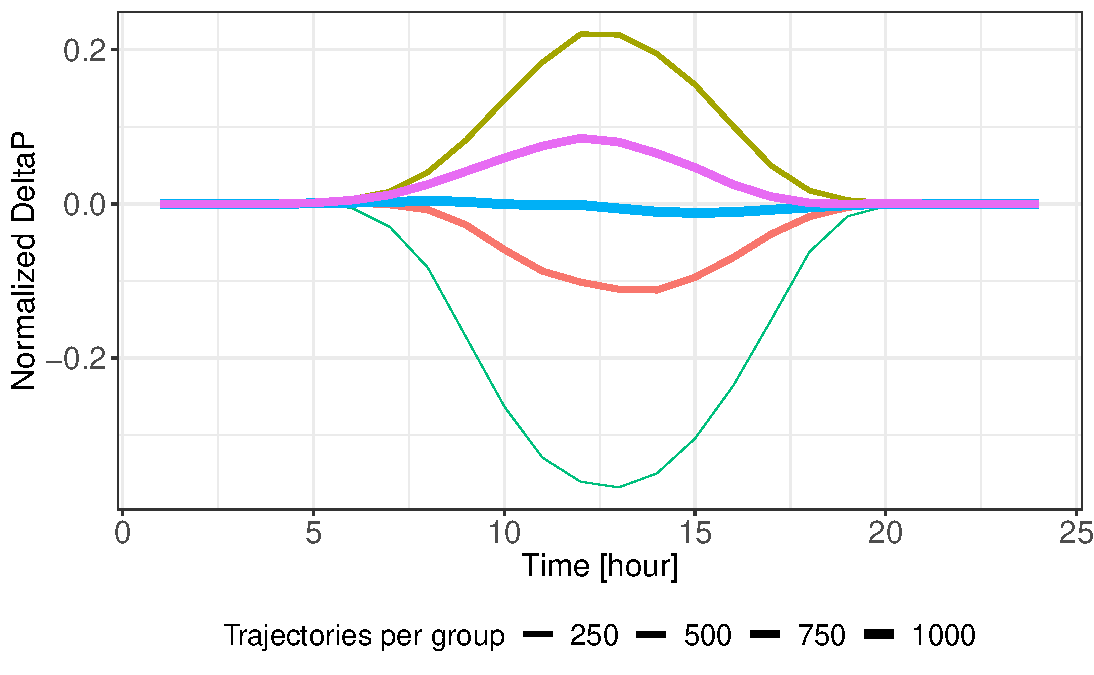
\includegraphics[width=0.9\linewidth]{Images/PV/Kmeans/Kmeans5Clusts.pdf} 
		\caption{5 clusters} 
		%\label{fig::HHMM_8HS_Traj_HS1} 
		%\vspace{4ex}
	\end{subfigure}%% 
	\begin{subfigure}[b]{0.5\linewidth}
		\centering
		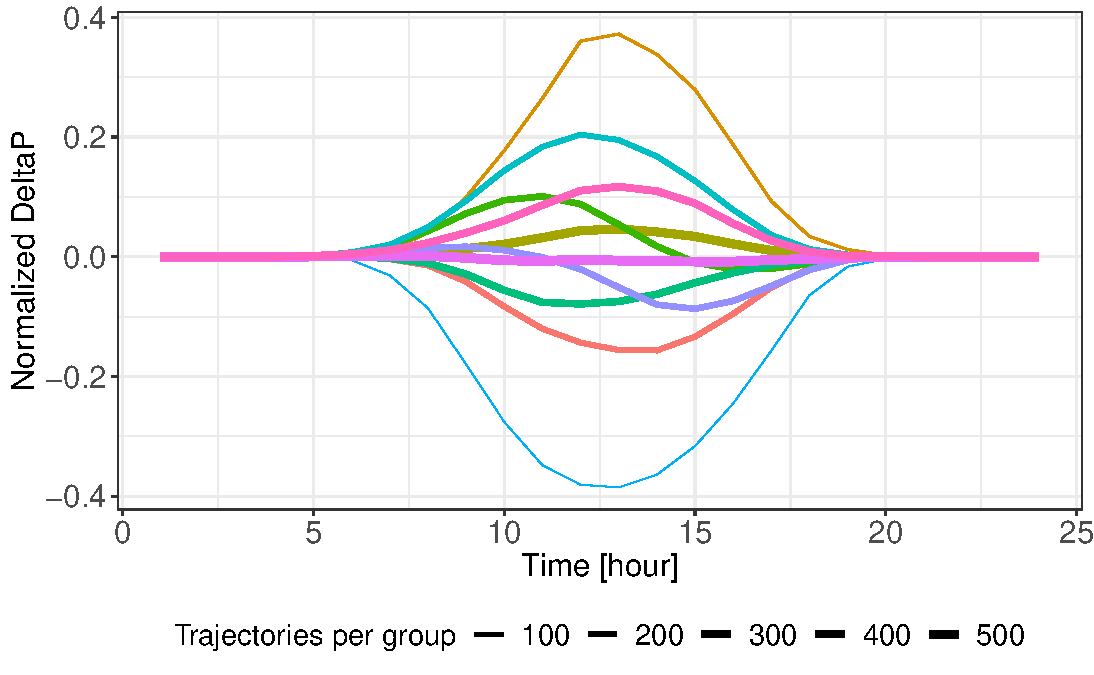
\includegraphics[width=0.9\linewidth]{Images/PV/Kmeans/Kmeans10Clusts.pdf} 
		\caption{10 clusters} 
		%\label{fig::HHMM_8HS_Traj_HS2} 
		%\vspace{4ex}
	\end{subfigure}
	
	\begin{subfigure}[b]{0.5\linewidth}
		\centering
		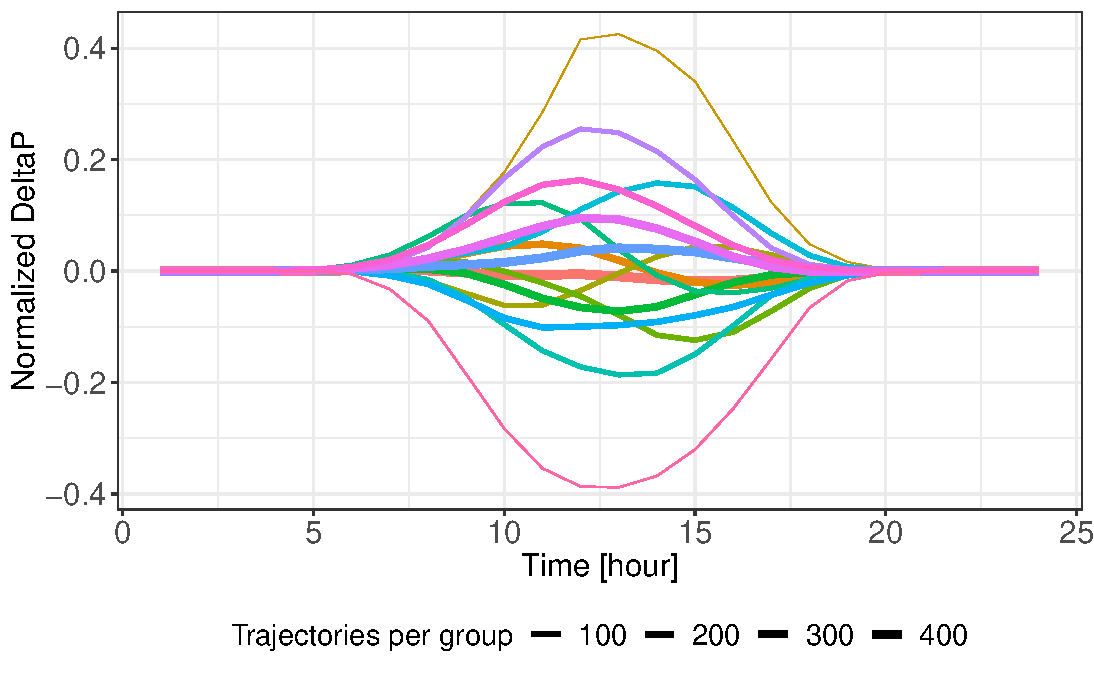
\includegraphics[width=0.9\linewidth]{Images/PV/Kmeans/Kmeans15Clusts.pdf} 
		\caption{15 clusters} 
		%\label{fig::HHMM_8HS_Traj_HS3} 
	\end{subfigure}%%
	\begin{subfigure}[b]{0.5\linewidth}
		\centering
		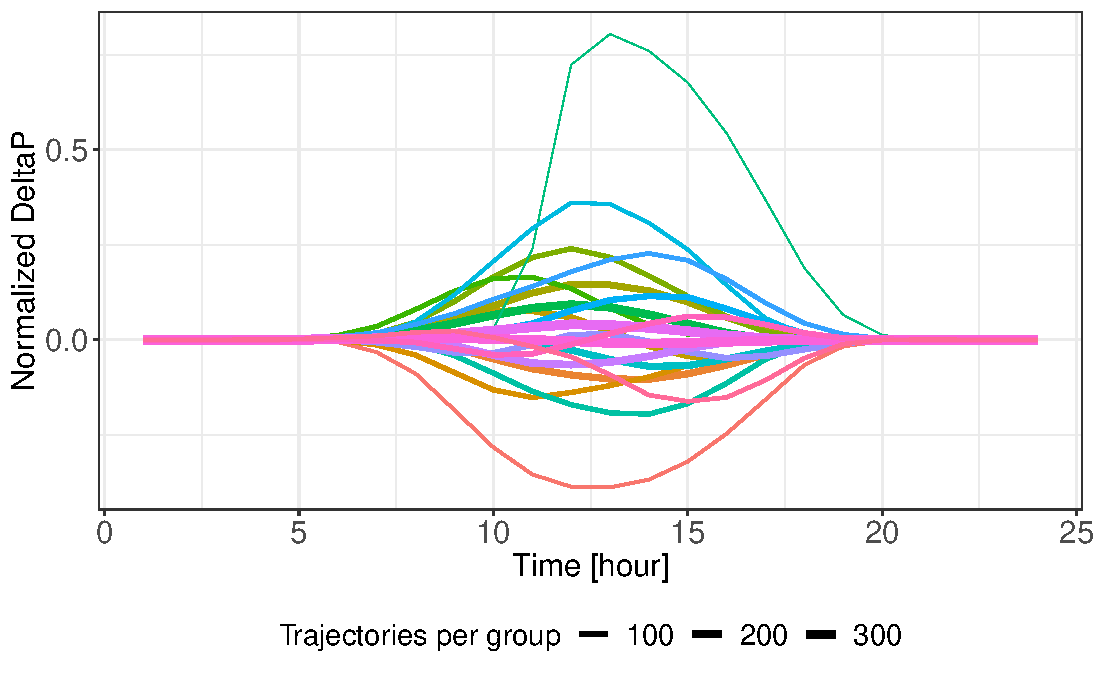
\includegraphics[width=0.9\linewidth]{Images/PV/Kmeans/Kmeans20Clusts.pdf} 
		\caption{20 clusters} 
		%\label{fig::HHMM_8HS_Traj_HS2} 
		%\vspace{4ex}
	\end{subfigure}
	
	\caption{Centroïdes des clusters obtenus par la méthode des Kmeans sur la série d'entraînement. la population des clusters est matérialisée par l'épaisseur du trait.}
	\label{fig:Kmeans_centers} 
\end{figure}

Dans cette section, une approche assez simple de la méthode des plus proche voisins a été mise en œuvre et elle a permis d'en démontrer le potentiel. En effet elle a permis d'atteindre des corrections des prévisions au cour de la journée qui permettant de réduire les erreurs de prévisions entre $25$ et $35\%$. De meilleurs résultats auraient probablement pu être obtenus en affinant la méthode. En effet, il aurait pu être intéressant de pondérer certaines heures dans l'identification des plus proches voisins afin de donner plus de poids aux dernières heures connues. Ou encore de regarder si la prise en compte du jour précédent pouvait amener de l'information supplémentaire ? Finalement, combiner l'utilisation de l'erreur absolue avec l'erreur quadratique aurait aussi pu amener plus d'informations. Cependant, le potentiel de cette méthode m'a conduit à explorer une autre piste. En effet, plutôt que de n'identifier que les trajectoires types via la méthode des Kmeans, de l'information supplémentaire sur les variances associées pouvaient se révéler utile en utilisant la méthode de mélange Gaussien.


\section{Résulats avec un GMM}
\label{sec:PV_GMM}

Le modèle de mélange Gaussien, présenté dans \ref{sec:Model_GMM}, a été ajusté sur la série temporelle des erreurs de prédiction photovoltaïques. Comme pour les Kmeans, il est nécessaire d'identifier le nombre optimal de clusters $K$. Pour ce faire, le critère BIC est à nouveau utilisé comme premier indicateur. On peut constater sur la figure \ref{fig:PV_GMM_BIC} que le modèle de type VII (matrice de variance covariance diagonale et à valeur unique par cluster) semble surpasser le modèle de type EII (matrice de variance covariance diagonale et à valeur unique commune pour tous les cluster). Cette figure ne présente pas les résultats obtenus par les autres modèles car ils n'ont pas convergé, probablement à cause d'un manque de données. En effet, même si le jeu d'entraînement se compose de 6 années complètes, cela ne représente qu'un total de $2190$ journées. Ce nombre est assez vite relativement faible face aux nombres de paramètres à estimer des GMM plus évolués (voir \ref{sec:Model_GMM}). Par exemple, si chaque valeur sur la diagonale est distincte alors on passe de $(K-1) + K\times d + K$ à $(K-1) + K\times d + K \times d$ paramètres et il est donc nécessaire d'avoir nettement plus de données pour les estimer. Dans ce contexte précis, il aurait pu être intéressant de pouvoir décrire la diagonale de la matrice de variance covariance par deux valeurs. Cela aurait pu permettre à l'algorithme de dissocier les variances pour les heures diurnes et nocturnes tout en restreignant le nombre de paramètres. Mais cette option n'est pas offerte par le package \texttt{Mclust} et n'a pas fait l'objet d'une implémentation de ma part par manque de temps.

\begin{figure}[h]
	\begin{subfigure}{0.5\linewidth}
		\centering
		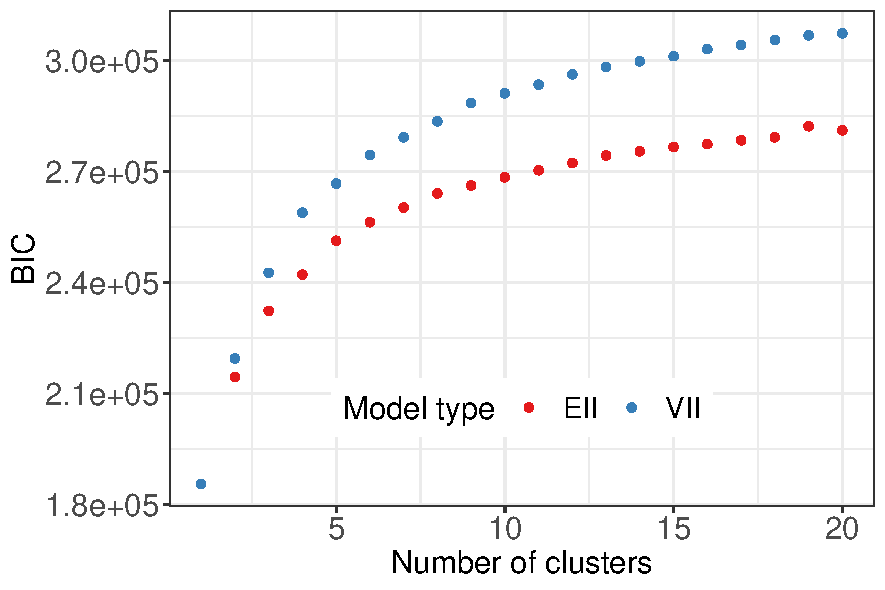
\includegraphics[width = 0.9 \linewidth]{Images/PV/GMM/GMM_BICCompare_20.pdf}
		\caption{Valeurs du critère BIC pour différents type de mélange gaussiens et nombres de groupes}
		\label{fig:PV_GMM_BIC}
	\end{subfigure}
	~
	\begin{subfigure}{0.5\linewidth}
		\centering
		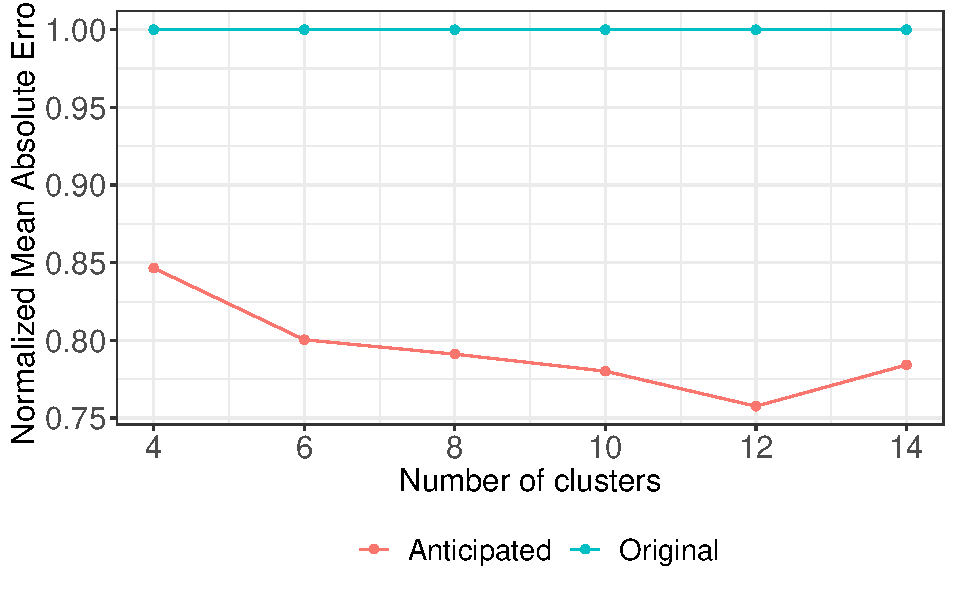
\includegraphics[width = 0.9 \linewidth]{Images/PV/GMM/GMM_CompareIntraday.pdf}
		\caption{Corrections d'erreurs à 10 heures obtenus avec plusieurs GMM dont le nombre de clusters $K$ diffèrent}
		\label{fig:PV_GMM_IntradayComp}
	\end{subfigure}
	\caption{Représentation de deux critères sur lesquels se sont basés le choix du nombre de groupes}
\end{figure}

Le critère BIC ne favorise pas un nombre spécifique de cluster mais donne plutôt une tendance générale favorisant systématiquement l'augmentation du nombre de clusters. Une explication plausible réside dans le fait que le phénomène sous-jacent, l'évolution du temps au sens météorologique du terme, est par définition un phénomène continu et non discret. Plus on discrétiserait son espace de représentation, plus on se rapprocherait d'une représentation continue et ainsi meilleurs sont les résultats. Afin de garder l'interprétabilité du modèle obtenu, et d'en limiter sa complexité, il est impératif de choisir un nombre de cluster relativement restreint. La figure \ref{fig:PV_GMM_BIC} montre une croissance plus faible en terme de critère BIC à partir du sixième cluster. Afin de combiner des informations provenant de deux indicateurs différents, il est possible de voir comment le GMM répond à une application spécifique en fonction de $K$. J'ai donc choisi de les comparer sur la base de leur potentiel à réaliser de la correction au cours de la journée. Des exemples de ces corrections sont présentées dans la figure \ref{fig:PV_GMM_IntraDay}. Ces résultats sont présentés sur la figure \ref{fig:PV_GMM_IntradayComp}. Un net gain, d'environ $5\%$, est constaté en passant de 4 clusters à 6. Ensuite les gains sont relativement plus faible et pour ré-obtenir un gain similaire il faudrait prendre 12 clusters. En comparant ces deux indicateurs, il semble que le modèle à 6 clusters soit un bon compromis entre complexité et précision.

\begin{figure}[h] 
	\begin{subfigure}[b]{0.5\linewidth}
		\centering
		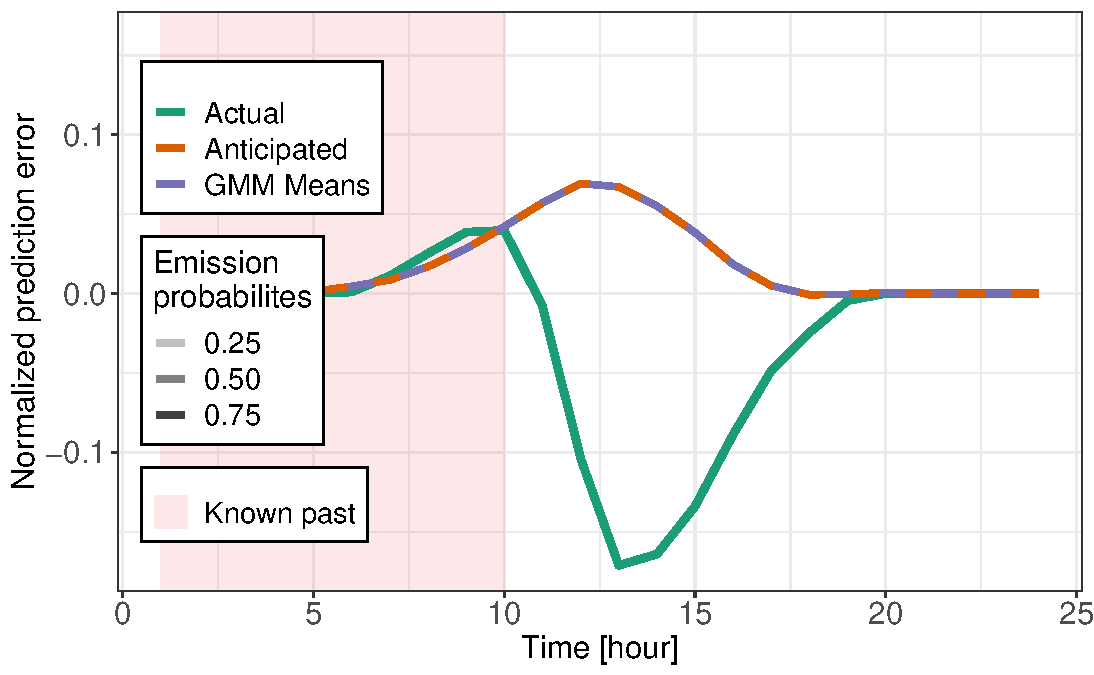
\includegraphics[width=0.9\linewidth]{Images/PV/GMM/GMM_6Clust_Intraday_24d_10h_idtest98.pdf} 
		%\caption{5 clusters} 
		%\label{fig::HHMM_8HS_Traj_HS1} 
		%\vspace{4ex}
	\end{subfigure}%% 
	\begin{subfigure}[b]{0.5\linewidth}
		\centering
		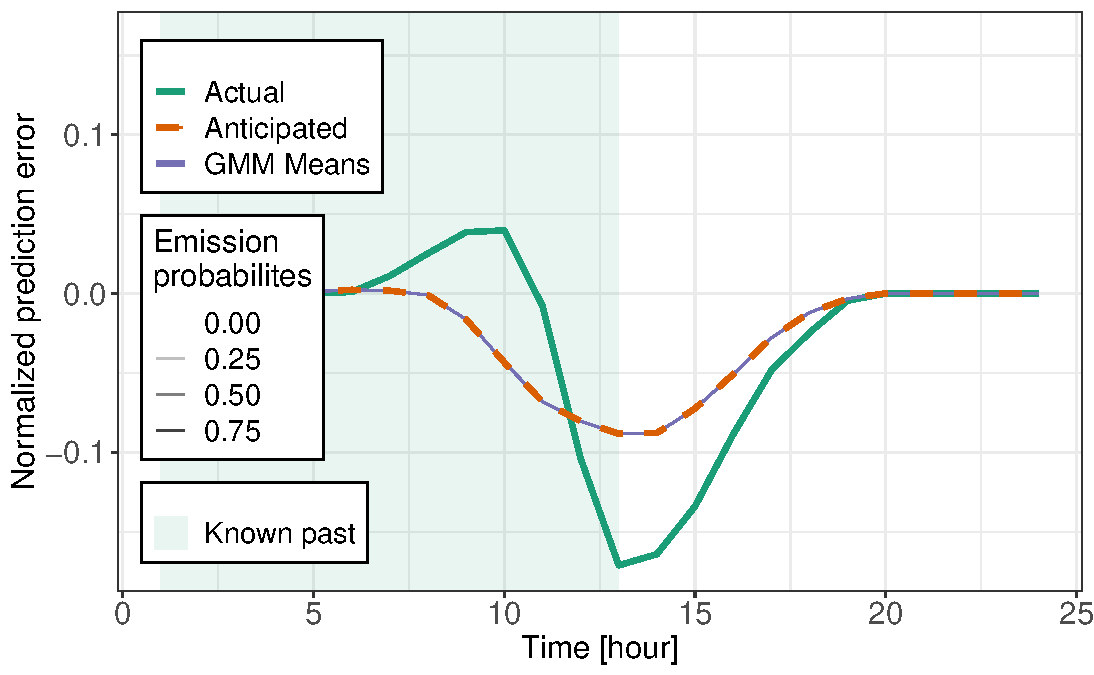
\includegraphics[width=0.9\linewidth]{Images/PV/GMM/GMM_6Clust_Intraday_24d_13h_idtest98.pdf} 
		%\caption{10 clusters} 
		%\label{fig::HHMM_8HS_Traj_HS2} 
		%\vspace{4ex}
	\end{subfigure}
	\centering
	\begin{subfigure}[b]{0.5\linewidth}
		\centering
		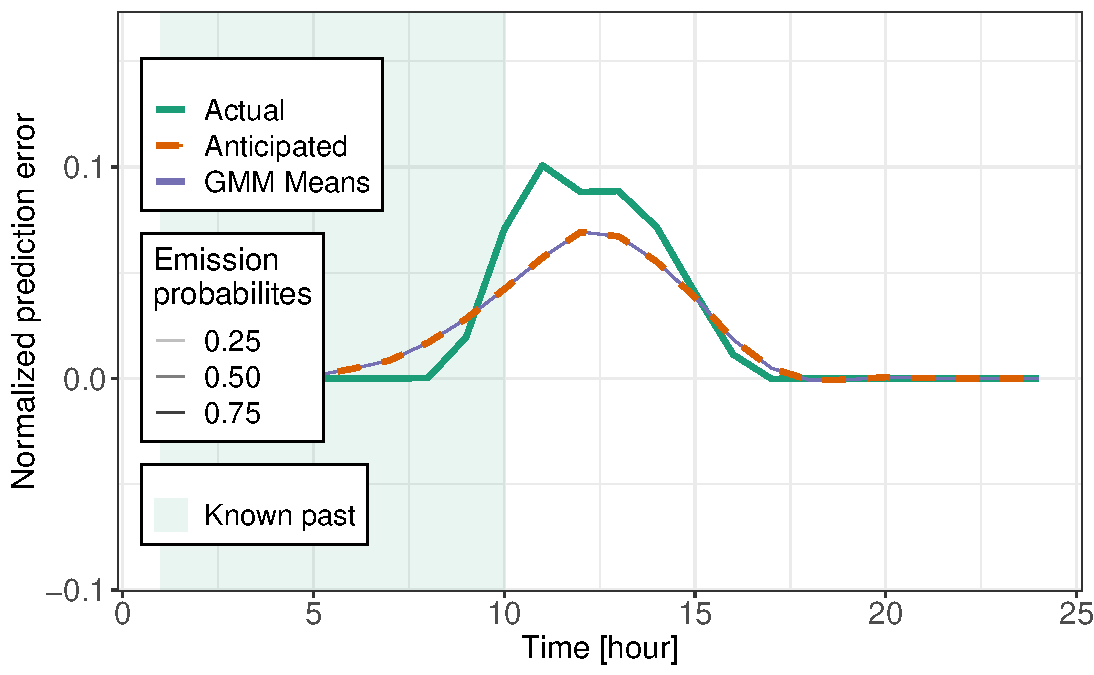
\includegraphics[width=0.9\linewidth]{Images/PV/GMM/GMM_6Clust_Intraday_24d_10h_idtest335.pdf} 
		%\caption{15 clusters} 
		%\label{fig::HHMM_8HS_Traj_HS3} 
	\end{subfigure}
	
	\caption{Corrections au cours de la journée avec le GMM de la figure \ref{fig:PV_GMM_MeanVarProp}. }
	\label{fig:PV_GMM_IntraDay} 
\end{figure}


Les paramètres du modèle obtenus sont présentés graphiquement dans la figure \ref{fig:PV_GMM_MeanVarProp}. Il est possible de constater que les trajectoires moyennes des états sont assez semblables à celles obtenus par la méthode des Kmeans (voir figure \ref{fig:Kmeans_centers}). Enfin, l'information supplémentaire réside dans la connaissance des variances pour chaque clusters. Elle sont relativement faible et globalement assez similaires les unes des autres pour les groupes allant de 1 à 5. Par contre, le groupe 6, a une variance nettement plus forte. Ce cluster, qui est significativement moins peuplé que les autres, regroupe les individus au comportement inhabituels et/ou chaotiques.

\begin{figure}[h]
	\centering
	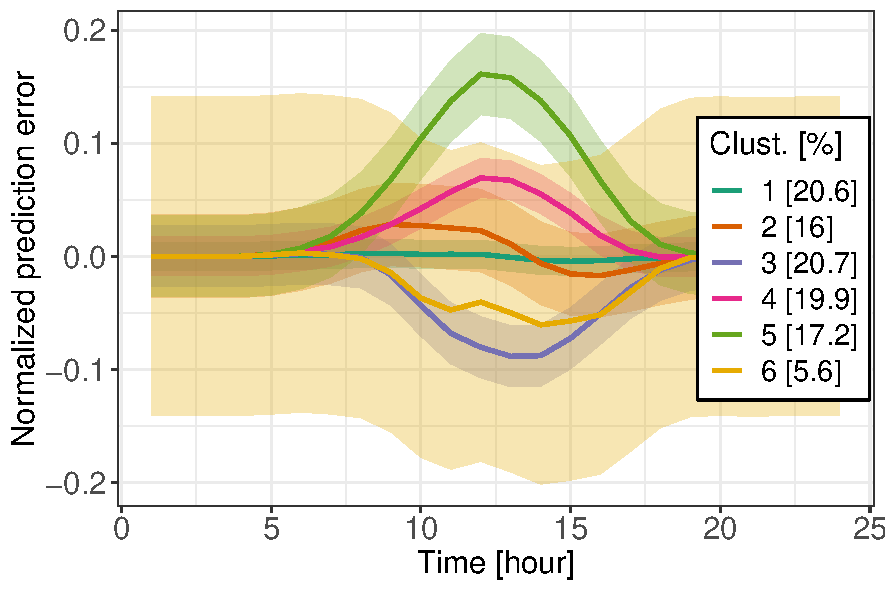
\includegraphics[width = 0.75 \linewidth]{Images/PV/GMM/GMM_MeansVars_6_dim24.pdf}
	\caption{Représentation graphique des paramètres du modèle GMM à 6 clusters obtenu sur la série des erreurs prévisions photovoltaïques. Les lignes continues représentent les moyennes, les fonds colorés leur intervalles de confiance de $68 \%$ respectifs. Les proportions respectives sont intégrées dans la légende.}
	\label{fig:PV_GMM_MeanVarProp}
\end{figure}


Finalement, l'utilisation de modèle GMM n'a pas permis d'améliorer les résultats obtenus en terme de corrections de prévisions au cours de la journée par rapport aux plus proches voisins. En effet, le modèle GMM retenu parvient à réduire de $20 \%$ les erreurs pour une correction à 10 heures alors que les plus proches voisins permettaient une réduction de l'ordre de $35 \%$. La variante en utilisant une identification de clusters type déterminés par la méthode des Kmeans conduisait à une réduction de l'odre de $25 \%$ dans les mêmes conditions. Cependant, le modèle GMM apporte quand même de l'information supplémentaire non négligeable avec les précisions sur les variances de chaque clusters. Ceci permet par exemple d'identifier les probabilités d'appartenance au cours de la journée via les densités de probabilités, ce qui est plus fiable que d'utiliser l'erreur absolue ou l'erreur quadratique. Par ailleurs, une fois les probabilités d'appartenance, cela permet de générer des scénarios de comportements sur le reste de la journée et ainsi de réaliser une prédiction stochastique sur le reste de la journée par opposition aux Kmeans qui proposaient une prévision déterministe. Mais, mis à part donner un comportement moyen, ce modèle ne permet toujours pas d'anticiper l'avenir au delà de la journée en cours. C'est pourquoi il pourrait être intéressant d'identifier un HMM dont la structure est similaire si ce n'est que la matrice de transition permette de prévoir des scénarios sur plusieurs journées.  

\section{Résultats avec un HMM}
\label{sec:PV_HMM}

\subsection{Détermination du modèle}

En gardant à l'esprit que ce modèle est identifié dans le but de générer des prévisions sur plusieurs journée, il est impératif de donner plus de liberté au HMM qu'au GMM quant à la structure de sa matrice de variance covariance. En effet, si on ne relaxe pas la contrainte d'avoir une valeur unique sur la diagonale de variance covariance alors le modèle ne sera jamais en mesure de capturer les erreurs nulles ou négligeables la nuit. Les scénarios générés n'auraient pas alors cette caractéristique et les performances en termes d'applications seraient grandement réduites. Cependant, ce faisant, le nombre de paramètres passe de chaque modèle devient alors :

\begin{equation}
\underbrace{K-1}_\text{Probabilités initiales}  + \underbrace{K \times d}_\text{Centres}  +  \underbrace{K \times d}_\text{Matrices de variance covariance} + \underbrace{K \times K}_\text{Matrice de transition}
\end{equation}

Par exemple, en prenant le cas d'une observation toutes les heures ($d=24$) et de 6 états cachés ($K=6$) par identification avec le GMM, il faut donc identifier $329$ paramètres. C'est donc plus du double des $155$ paramètres du GMM sélectionné dans la section \ref{sec:PV_GMM}. Pour pallier à ce problème, j'ai procédé à une réduction de dimension de l'espace par la méthode de l'ACP (voir \ref{sec:Model_ACP}). Les résultats obtenus en fonction du nombre de composantes sélectionnées sont présentés dans la figure \ref{fig:PV_HMM_ACP_DimSelect}. J'ai choisi de garder un nombre de composante principales expliquant $99 \%$ de la variance totale, soit 6 composantes principales. 

\begin{figure}[h]
	\centering
	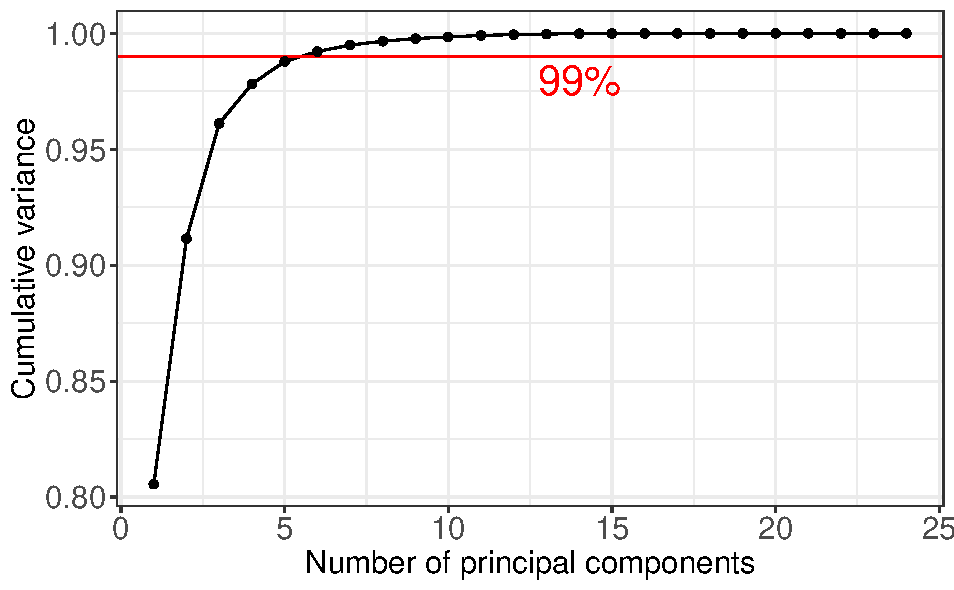
\includegraphics[width = 0.6 \linewidth]{Images/PV/ACP/ACP_DimSelect.pdf}
	\caption{Variance cumulée expliquée en fonction du nombre de composante principales}
	\label{fig:PV_HMM_ACP_DimSelect}
\end{figure}

Ces 6 composantes sont présentées sur la figure \ref{fig:PV_HMM_ACP_PC}. Les 6 composantes principales partagent le fait d'être nulles ou négligeables avant 5 heures et après 20 heures. Ces plages horaires sont celles pour lesquelles les erreurs de prédiction sont nulles toute l'année comme le montre la figure \ref{fig:Donnees_TenneT_Bayern_BoxHist}. La première composante, si multipliée par le facteur adéquat, peut permettre de représenter la plupart des trajectoires types obtenues par les différents modèles des sections précédentes. On comprend donc pourquoi elle permet, à elle seule, d'expliquer $80\%$ de la variance. Physiquement, elle traduit une pure sur ou sous estimation de la puissance productible au jour considéré. La deuxième composante principale cherche à représenter les journées avec surestimation le matin et sous estimation l'après-midi et inversement. Certaines trajectoires types obtenues précédemment traduisaient la relativement forte présence de journées d'erreurs de prévision avec ce profil. Les composantes principales d'ordres supérieurs ajoutent à chaque fois une alternance entre surestimation et sous-estimation. Procéder à une ACP dans le cas présent revient donc à faire décomposition en série de Fourier sur la plage d'heures ensoleillées tout en laissant toujours nulles les heures qui ne le sont jamais.

\begin{figure}[h]
	\centering
	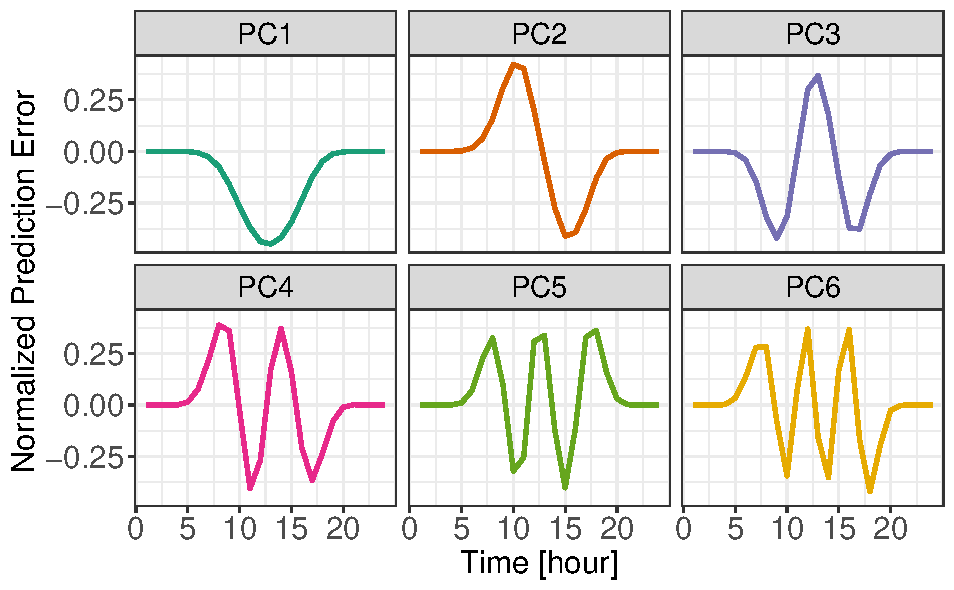
\includegraphics[width = 0.8 \linewidth]{Images/PV/ACP/ACP_PrincipalComp_6.pdf}
	\caption{Représentation graphique des 6 composantes principales obtenues par la l'ACP dans l'espace d'origine de dimension 24}
	\label{fig:PV_HMM_ACP_PC}
\end{figure}

Dans cet espace réduit, le nombre de paramètres d'un HMM à états cachés ne serait donc plus que de $113$ contre les $329$ dans l'espace de départ. L'initialisation des paramètres pour le HMM a été faite à partir de ceux obtenus pour le GMM. Les paramètres du modèle obtenu sont présentés graphiquement dans la figure \ref{fig:PV_HMM_MeanVarACP}.


\begin{figure}[h] 
	\begin{subfigure}[b]{0.5\linewidth}
		\centering
		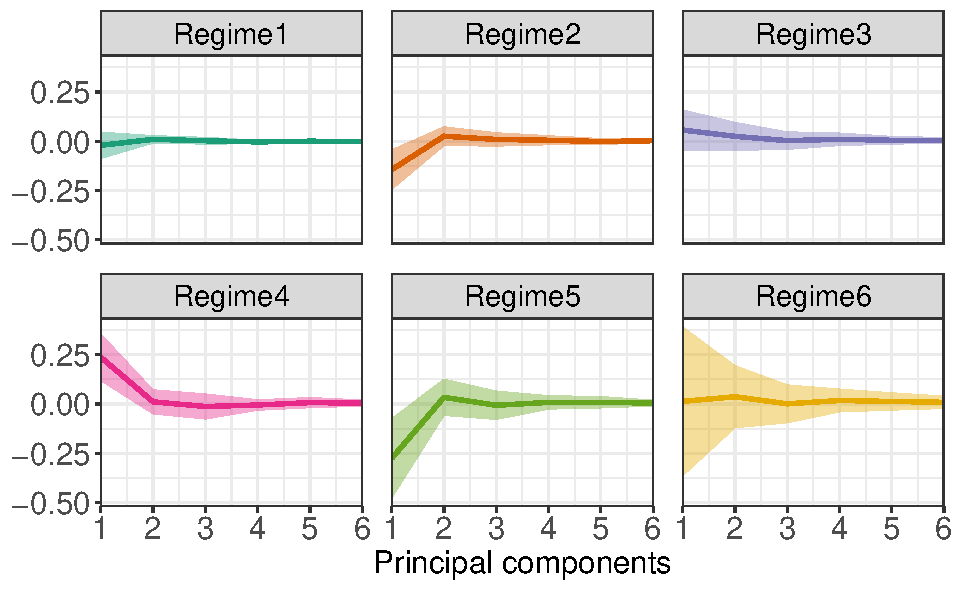
\includegraphics[width = 0.95 \linewidth]{Images/PV/HMM/MS6AR_6dimACP.pdf}
		\caption{Espace réduit}
		\label{fig:PV_HMM_MeanVarACP}
		%\vspace{4ex}
	\end{subfigure}%% 
	\begin{subfigure}[b]{0.5\linewidth}
		\centering
		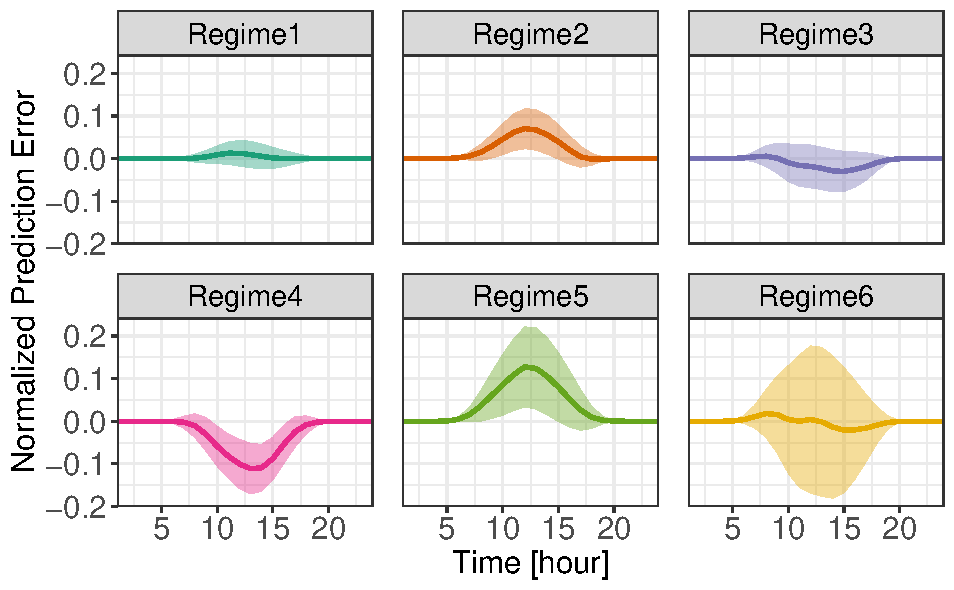
\includegraphics[width = 0.95 \linewidth]{Images/PV/HMM/MS6AR_24dimReco.pdf}
		\caption{Espace original}
		\label{fig:PV_HMM_MeanVarOrig}
		%\vspace{4ex}
	\end{subfigure}
	
	\caption{Représentation des moyennes et variances d'un HMM à 6 états cachés}
	\label{fig:PV_GMM_MeanVar_OrigACP} 
\end{figure}

%\begin{figure}[h]
%	\centering
%	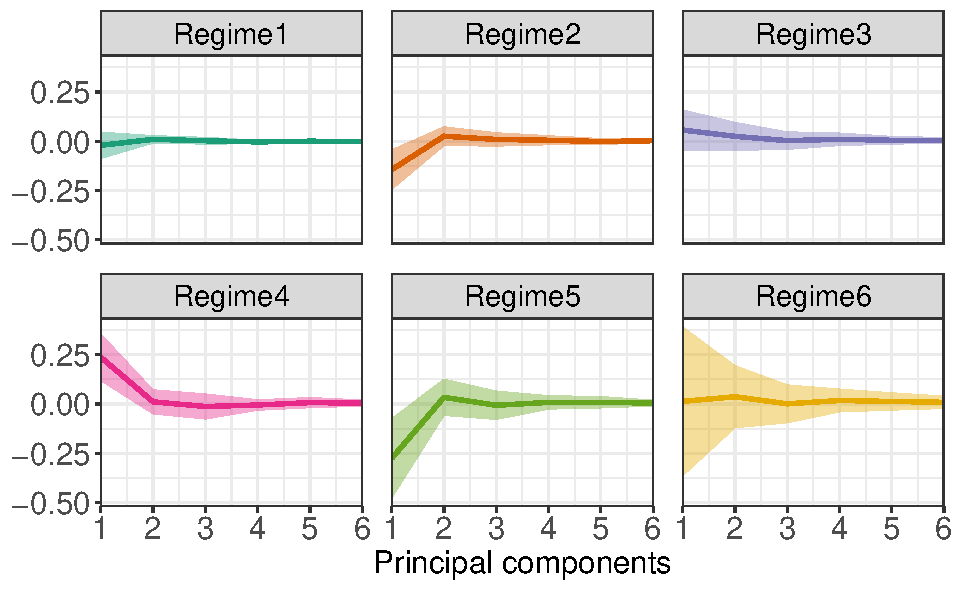
\includegraphics[width = 0.8 \linewidth]{Images/PV/HMM/MS6AR_6dimACP.pdf}
%	\caption{Représentation des 6 états cachés obtenus pour un HMM à 6 états cachés dans l'espace de dimension réduite}
%	\label{fig:PV_HMM_MeanVarACP}
%\end{figure}

L'interprétation des régimes sous cette forme n'est pas aisée mais deux éléments sont intéressant à noter. Tout d'abord, les régimes sont caractérisés par des valeurs non négligeables sur la première composante uniquement. D'autre part, la variance diminue en augmentant l'ordre de la composante principale, et ce dans tous les régimes. Ce phénomène est inhérent à l'utilisation de l'ACP qui détermine les composante principales en s'appuyant sur une maximisation de la variance qu'elles expliquent. Les régimes, transformés dans l'espace d'origine, sont présentés dans la figure \ref{fig:PV_HMM_MeanVarOrig}. On retrouve les profils obtenus dans par les modèles utilisés précédemment. Notamment deux modèles de surestimation plus ou moins forte, deux modèles de sous-estimation plus ou moins forte et deux modèles à moyenne nulles mais avec des variances très distinctes. Comme dans le cas du GMM, le régime 6 sert à caractériser les journées aux profils atypiques. 

\todo{Présenter la matrice de transition aussi !}

\subsection{Caractérisation statistique du modèle}
Une particularité des HMM est qu'ils permettent facilement de générer des données synthétiques. En effet, une fois l'initialisation faite, la matrice de transition et les paramètres des états cachés contiennent l'information nécessaire à la production de données synthétiques de la longueur voulue. La figure \ref{fig:PV_HMM_Stat_Zoom} montre une portion de série synthétique dont le profil des journées paraît cohérent avec ce qui est présenté dans la figure \ref{fig:Data_PV_PredErrs}. Il est alors possible de comparer des critères statistiques sur ces données synthétiques et sur la série originale pour évaluer le caractéristiques capturées ou non par le modèle. La figure \ref{fig:PV_HMM_Stat_QQ} montre le diagramme quantile-quantile des séries synthétiques et de la série originale. Pour rappel, ce diagramme cherche à représenter les quantiles d'une série par rapport à ceux de l'autre. Si ces deux séries sont émises par la même distribution, alors les quantiles s'alignent tous sur une droite. Sur cette figure on peut voir que les quantiles s'alignent parfaitement sur l'intervalle $[-0.25,0.25]$ qui, d'après la figure \ref{fig:Data_TenneT_Bayern_BoxHist} représente une grande majorité des observations. Cependant, la figure indique clairement que le modèle ne réussit pas à capturer les queues de la distribution en sous estimant l'occurence de prévision très mauvaises.

\begin{figure}[h] 
	\begin{subfigure}[b]{0.5\linewidth}
		\centering
		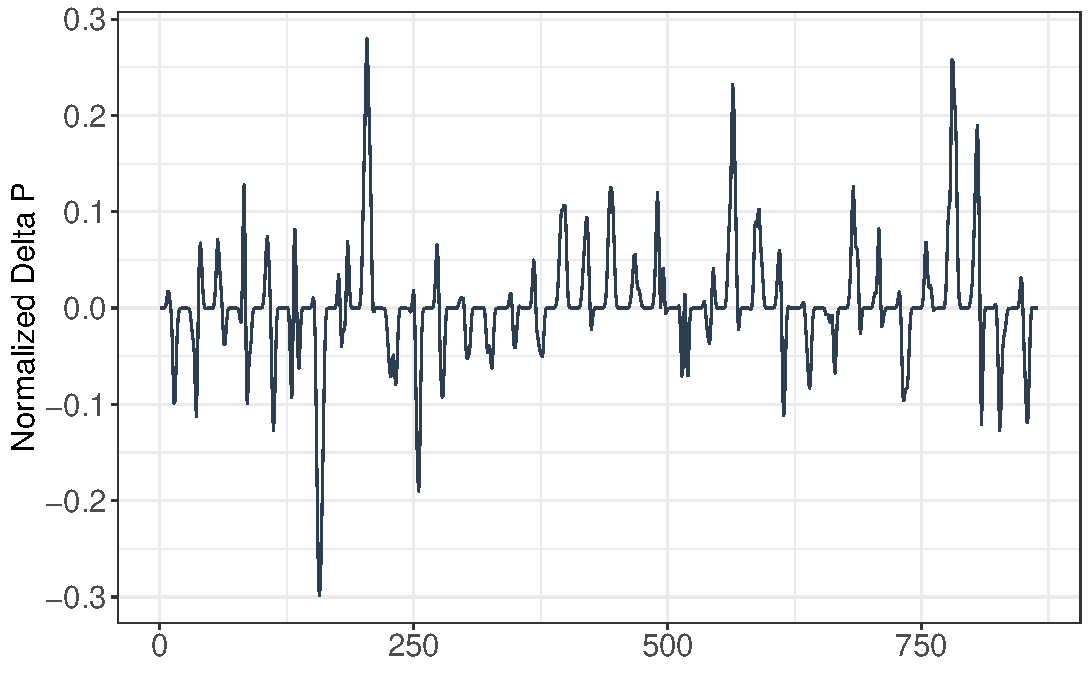
\includegraphics[width = 0.95 \linewidth]{Images/PV/HMM/Stats/SyntheticDataZoom.pdf}
		\caption{Espace réduit}
		\label{fig:PV_HMM_Stat_Zoom}
		%\vspace{4ex}
	\end{subfigure}%% 
	\begin{subfigure}[b]{0.5\linewidth}
		\centering
		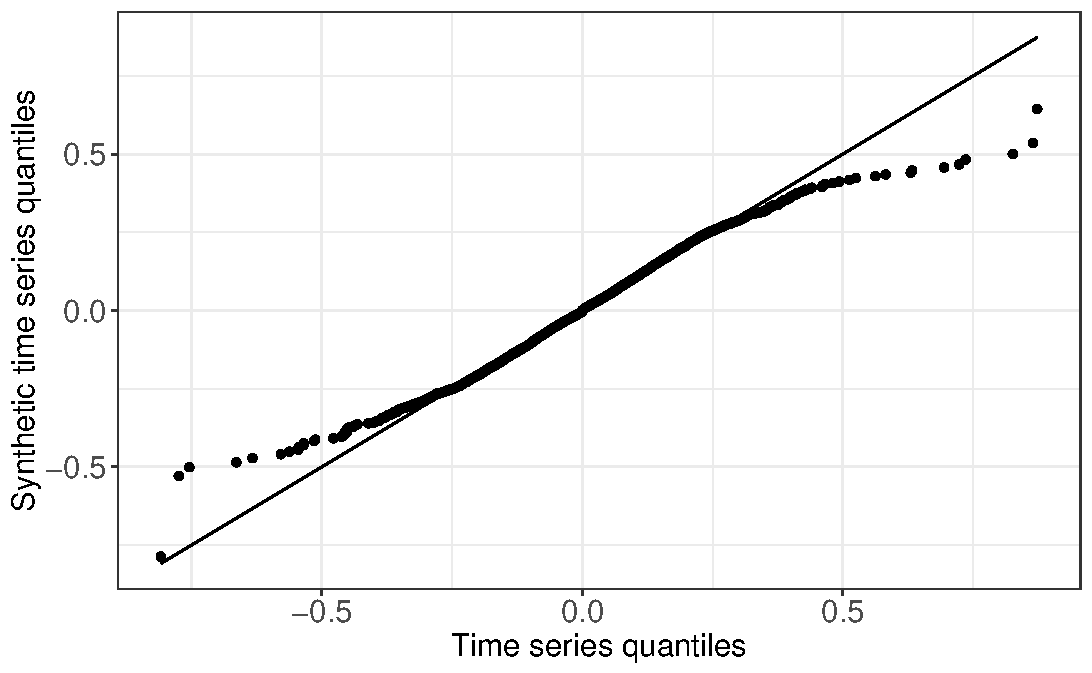
\includegraphics[width = 0.95 \linewidth]{Images/PV/HMM/Stats/QQPlot.pdf}
		\caption{Espace original}
		\label{fig:PV_HMM_Stat_QQ}
		%\vspace{4ex}
	\end{subfigure}
	
	\caption{Représentation des moyennes et variances d'un HMM à 6 états cachés}
	\label{fig:PV_HMM_Stat_ZoomQQ} 
\end{figure}

La figure \ref{fig:PV_HMM_Stat_MDO} représente le temps de séjour moyen au dessus d'une valeur seuil. Cette valeur caractérise la dynamique globale de la série considérée. On remarque une nette diminution dans le temps de séjour moyen autour de 0. Ceci s'explique par la présence des erreurs nulles la nuit. En effet, en considérant une valeur seuil très légèrement positive, alors le temps de séjour moyen peut encore être assez élevé en présence de journée de sous-estimation (d'erreurs négatives). En considérant maintenant une valeur seuil très légèrement négative, elle sera nécessairement dépassée positivement à la prochaine période nocturne. Ce faisant le temps de séjour moyen au dessus de cette valeur seuil sera, au maximum, égal à la durée de l'ensoleillement à la période considérée. Cette particularité semble être parfaitement capturée par le modèle avec une superposition des temps de séjours des séries synthétiques et de la série originale sur cet intervalle. On retrouve une bonne superposition sur l'intervalle $[-0.25,0.25]$ et même un petit peu au delà. Les sous estimations des événements menant à des prédictions de mauvaises qualités se retrouvent aussi sur ce graphique. Cependant, l'écart de comportement sur les marges entre la série originale et la série synthétique est magnifié par l'échelle logarithmique. La figure \ref{fig:PV_HMM_Stat_NU} montre le nombre de dépassement positifs de valeurs seuils et traduit donc la volatilité des séries. Selon cette métrique il y a superposition presque parfaite entre les séries synthétiques et la série originale, ce qui traduit que le modèle capture avec succès la volatilité de la série temporelle.

\begin{figure}[h] 
	\begin{subfigure}[b]{0.5\linewidth}
		\centering
		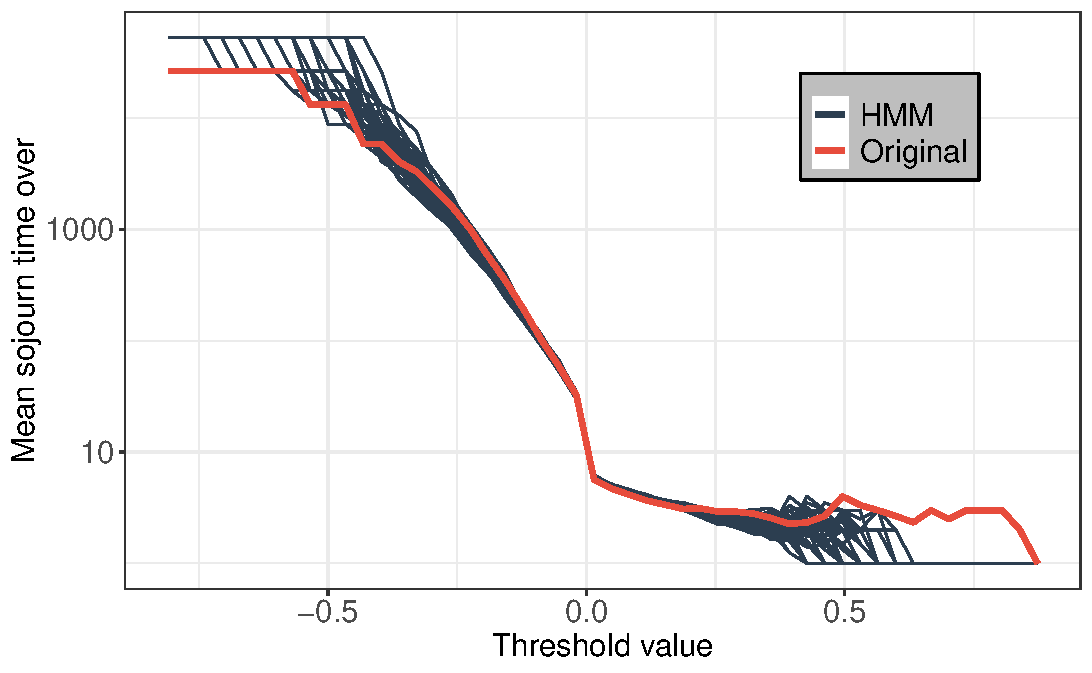
\includegraphics[width = 0.95 \linewidth]{Images/PV/HMM/Stats/MDO.pdf}
		\caption{Temps de séjour moyen au dessus d'une valeur seuil}
		\label{fig:PV_HMM_Stat_MDO}
		%\vspace{4ex}
	\end{subfigure}%% 
	\begin{subfigure}[b]{0.5\linewidth}
		\centering
		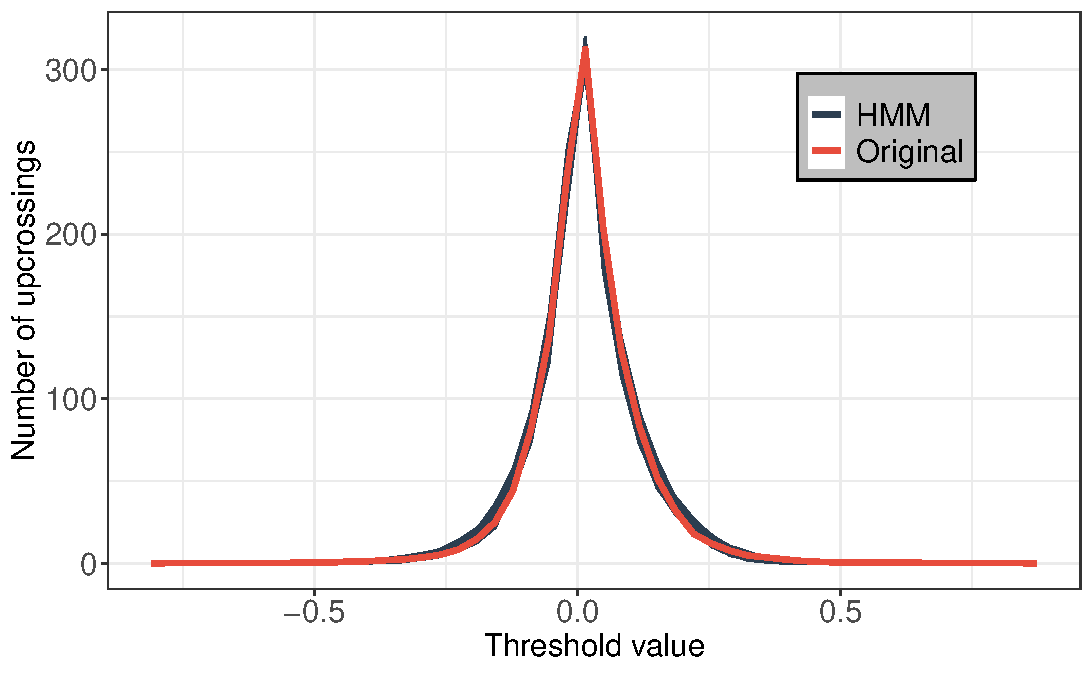
\includegraphics[width = 0.95 \linewidth]{Images/PV/HMM/Stats/NU.pdf}
		\caption{Nombre de dépassement positifs}
		\label{fig:PV_HMM_Stat_NU}
		%\vspace{4ex}
	\end{subfigure}
	
	\caption{Caractérisation statistiques par rapport à des valeurs seuils}
	\label{fig:PV_HMM_Stat_MDONU} 
\end{figure}

Cependant ces métriques ne parviennent pas à mettre en évidence deux sources de différences entre la série originale et la série synthétique. Tout d'abord, au vu des profils moyens du modèle et matrices de variances covariances, peu ou pas de journée avec une inversion de profil ne sont générées. Ce ne sont pas les profils les plus typiques, mais la méthode des Kmeans les exhibait à partir de 7 ou 8 clusters. D'autre part, il s'agit ici de statistiques réalisées sur l'ensemble de la série et qui ne tiennent donc pas compte de particularismes saisonniers. Il serait donc intéressant de réaliser ces statistiques sur des périodes de l'année et de voir si les résultats diffèrent. Le cas échéant, la prise en compte de la date calendaire par le modèle HMM serait une évolution non négligeable.




%\begin{figure}[h]
%	\centering
%	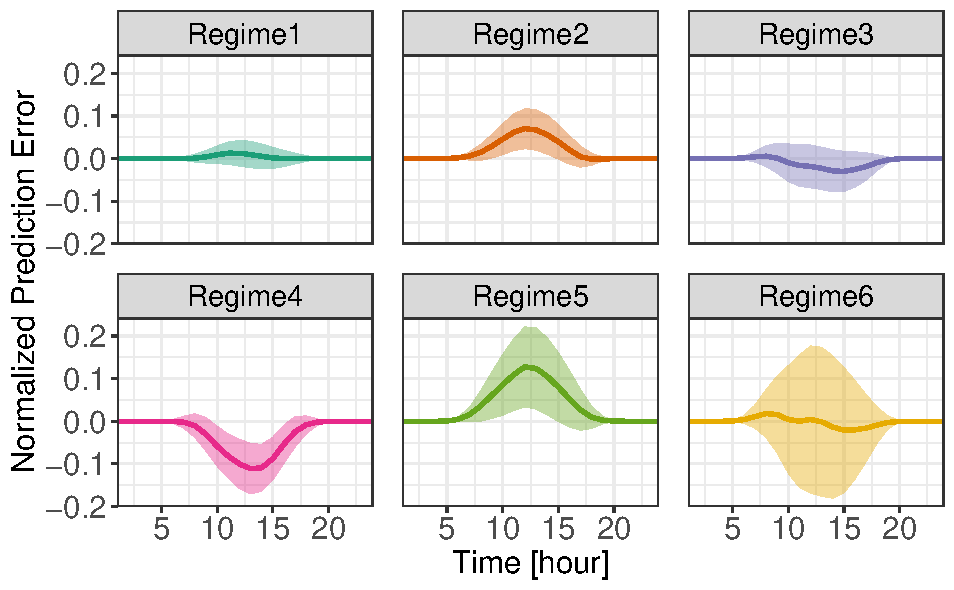
\includegraphics[width = 0.8 \linewidth]{Images/PV/HMM/MS6AR_24dimReco.pdf}
%	\caption{Représentation des 6 états cachés obtenus pour un HMM à 6 états cachés dans l'espace original}
%	\label{fig:PV_HMM_MeanVarOrig}
%\end{figure}

\subsection{Applications du modèle}

Utiliser ce modèle pour faire de la correction au cours de la journée n'apporterait que peu de gain par rapport au GMM de la section \ref{sec:PV_GMM} au vu de leurs nombreuses similitudes. Cependant, il est possible de l'utiliser pour faire des prévisions d'ensembles sur une ou plusieurs journées. Comme pré-requis, il est nécessaire de pouvoir déterminer les probabilités d'appartenance d'une journée à chacun des états cachés. Elles sont déterminées par l'utilisation de l'algorithme forward backward décrit dans \ref{subsubsec:Models_HMM_Apprentissage}. Des exemples de probabilités d'appartenance sont présentées dans la figure \ref{fig:PV_HMM_Forward} dans l'espace réduit (figure \ref{fig:PV_HMM_ForwardReduct}) et dans l'espace d'origine (figure \ref{fig:PV_HMM_ForwardOrig}).

\begin{figure}[h]
	\begin{center}
		
		\begin{subfigure}[b]{0.5\linewidth}
			\centering
			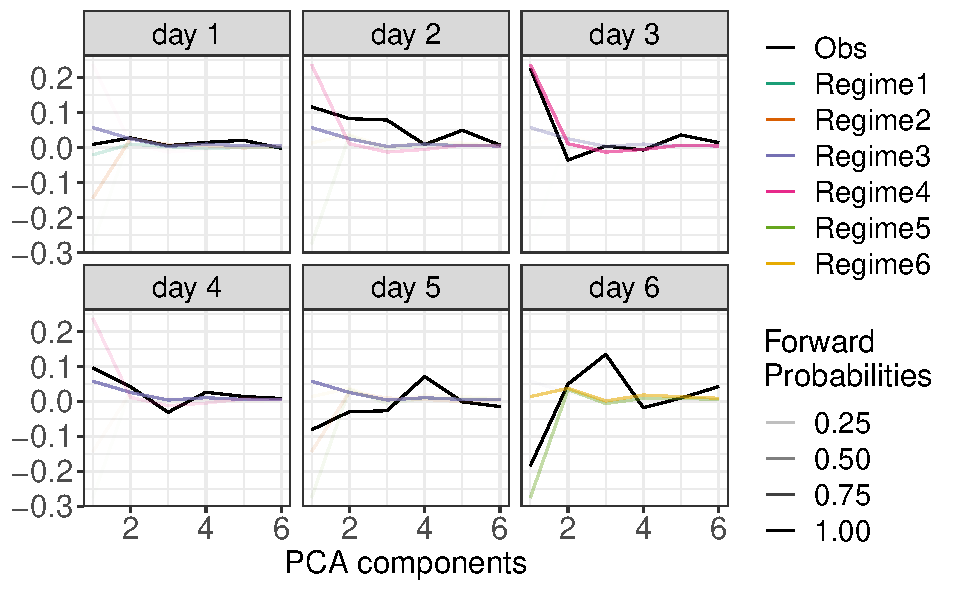
\includegraphics[width = 0.95 \linewidth]{Images/PV/HMM/HMM_ForwardProb_ACP_TrainDataset.pdf}
			\caption{Espace réduit}
			\label{fig:PV_HMM_ForwardReduct}
			%\vspace{4ex}
		\end{subfigure}%%
		~
		\begin{subfigure}[b]{0.5\linewidth}
			\centering
			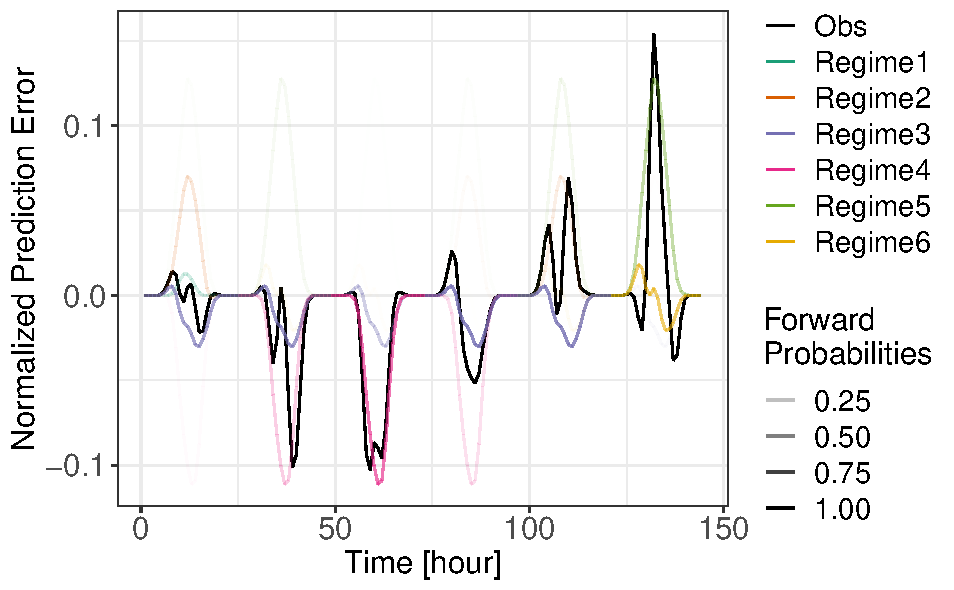
\includegraphics[width = 0.95 \linewidth]{Images/PV/HMM/HMM_ForwardProb_Reconstructed_TrainDataset.pdf}
			\caption{Espace original}
			\label{fig:PV_HMM_ForwardOrig}
			%\vspace{4ex}
		\end{subfigure}
	\end{center}
	
	\caption{Probabilités d'appartenance de 6 jours consécutifs aux états du modèle présenté dans la figure \ref{fig:PV_GMM_MeanVar_OrigACP}}
	\label{fig:PV_HMM_Forward} 
\end{figure}

On constate que, dans cet exemple, les probabilités d'appartenance mettent en évidence une compétition entre plusieurs états. En effet, comme aucune des trajectoires ne correspond exactement à une trajectoire type, c'est l'information sur les variances de chaque états qui est prépondérante. Par exemple, le profil moyen de la première journée semble, dans l'espace de dimension réduit, être le plus proche du Régime 1. Cependant, comme il a une très faible variance notamment sur les composantes principales d'ordre supérieur à 1, il n'a pas une plus grande probabilité d'avoir émis cette observation que les régimes 2 et 3. La troisième journée se rapproche très fortement de la trajectoire moyenne du régime 4 et il est donc nettement plus probable que ce soit lui qui ait la probabilité d'émission la plus forte. La sixième journée représente un autre cas intéressant. En effet, la première composante principale est assez proche de celle de l'état 5. Mais, au vu de la forte valeur sur la troisième composante principale, une compétition entre le régime 5 (forte erreurs positive) et le régime 6 (caractérisé par sa forte variance) s'installe.

A partir de ces probabilités d'appartenance, il est possible de faire de la prévision d'ensemble, c'est à dire de la génération de scénarios probables. En effet, en les utilisant pour définir une loi de probabilité multinomiale, il est possible de déterminer pour chaque scénario le régime ayant généré la trajectoire initiale. Le régime suivant est alors déterminé par tirage d'une autre loi binomiale définie cette fois par une ligne de la matrice de transition $\Gamma$. L'observation générée sera donc la moyenne du régime tiré auquel est ajouté un bruit définit par la matrice de variance covariance dudit régime. L'opération est à répéter jusqu'à l'obtention de scénarios de la durée voulue. La figure \ref{fig:PV_HMM_Scenarios} montre des exemples de scénarios générés dans 4 situations différentes.

\begin{figure}[h]
	\begin{center}
		
		\begin{subfigure}[b]{0.5\linewidth}
			\centering
			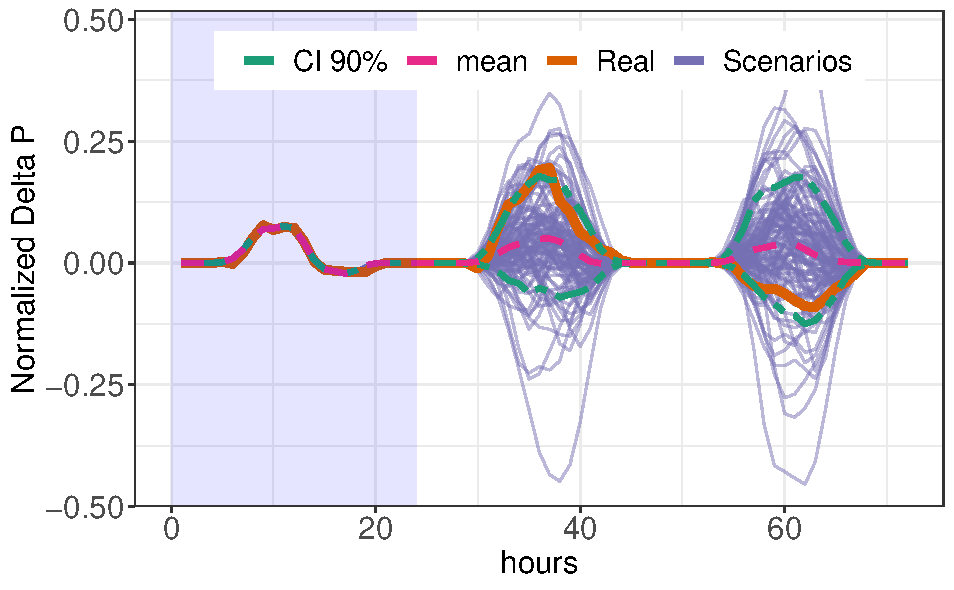
\includegraphics[width = 0.95 \linewidth]{Images/PV/HMM/id175.pdf}
			\caption{25-27 Juin 2017}
			%\vspace{4ex}
		\end{subfigure}%%
		\begin{subfigure}[b]{0.5\linewidth}
			\centering
			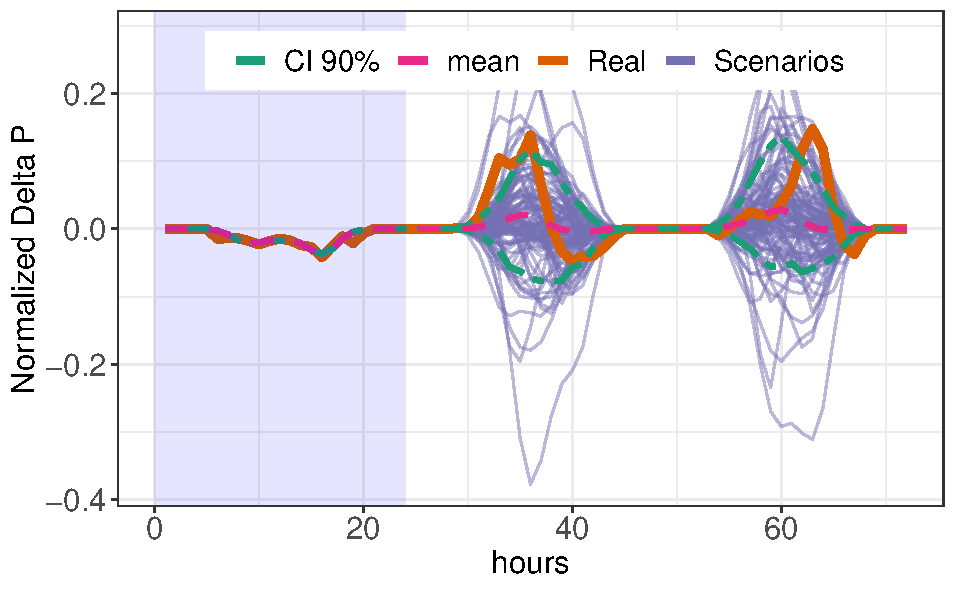
\includegraphics[width = 0.95 \linewidth]{Images/PV/HMM/id187.pdf}
			\caption{7-9 Juillet 2017}
			%\vspace{4ex}
		\end{subfigure}
		
		\begin{subfigure}[b]{0.5\linewidth}
			\centering
			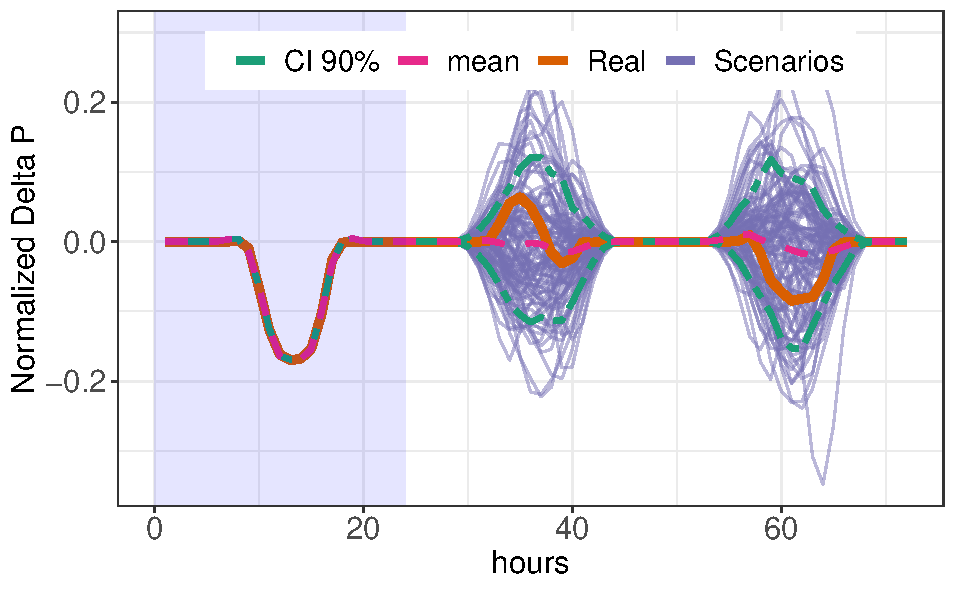
\includegraphics[width = 0.95 \linewidth]{Images/PV/HMM/id27.pdf}
			\caption{27-29 Janvier 2017}
			%\vspace{4ex}
		\end{subfigure}%%
		\begin{subfigure}[b]{0.5\linewidth}
			\centering
			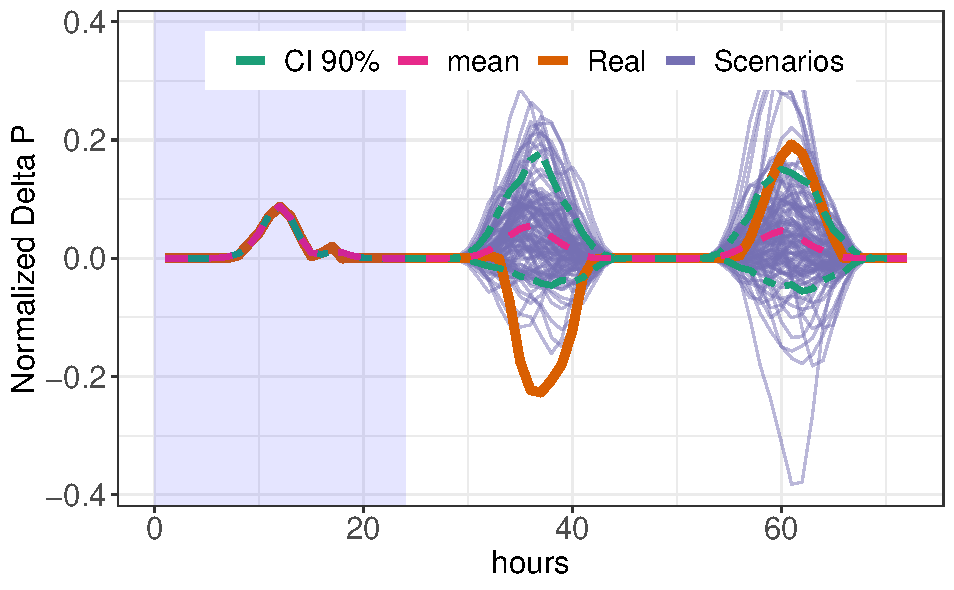
\includegraphics[width = 0.95 \linewidth]{Images/PV/HMM/id41.pdf}
			\caption{10-12 février 2017}
			%\vspace{4ex}
		\end{subfigure}
	\end{center}
	
	\caption{Génération de 10 scénarios à partir d'initialisations différentes matérialisées par un fond coloré. Les différents scénarios sont en violet, leur moyenne en rose, leur intervalle de prévision à $90\%$ en vert et enfin la série originale en orange.}
	\label{fig:PV_HMM_Scenarios} 
\end{figure}

Il est intéressant de constater que dans presque tous les cas, la série originale est bien intégrée dans le faisceau de scénarios. Cependant le 10 février illustre comment tous les scénarios prédits sont positifs ou presque alors que l'erreur réellement observée est négative. Par ailleurs, il est important de remarquer comment l'initialisation, traduite par des probabilités d'appartenance, influe le faisceau de scénarios générés. On constate par exemple que l'initialisation du 27 Janvier donne lieu a des scénarios équitablement positifs ou négatifs et de faible amplitude. En effet parmi les 100 scénarios, très peu sortent de l'intervalle des $20\%$ d'erreurs. Le 25 Juin et le 10 février génèrent quant à eux des scénarios de relativement faible amplitude mais en très grosse majorité positifs.

Afin de caractériser ces ensembles de prédictions, \cite{madsen_protocol_nodate} préconise l'utilisation d'au moins trois critères, à savoir la MAE (\ref{subsec:Model_Metric_MAE}), l'erreur quadratique (\ref{subsec:Model_Metric_RMSE}) et l'erreur moyenne (\ref{subsec:Model_Metric_BIAS}).


\begin{table}[h]
\centering
\caption{Score obtenus par différents modèles pour la simulation de 100 scénarios}
\begin{tabular}{lccc}
	& MAE  & RMSE & BIAS \\
HMM	& $2.049374 \times 10^{-2}$ & $4.680091\times 10^{-2}$ & $1.05063 \times 10^{-2}$	    \\
SARIMA	&  &  & 
\end{tabular}
\end{table}

   

\chapter{Conclusion et perspectives}
Au cours de ce stage, j'ai eu l'occasion d'étudier des séries d'erreurs de prévision de production d'énergie d'origine solaire et photovoltaïque. Côté éolien, leur étude avait déjà montré un potentiel intéressant à travers l'étude réalisée par \cite{haessig_dimensionnement_2014} et la mise en place d'un modèle AR(1). Côté photovoltaïque, \cite{latimier_gestion_2016} avait identifié la présence de profils typiques dans les données et proposé l'idée d'une approche par trajectoire. Dans les deux cas, l'objectif de ce stage était de poursuivre les pistes ouvertes dans ces deux directions afin de voir si des modèles plus complexes pouvaient améliorer les résultats.

Concernant les erreurs de prévision de production éolienne, un modèle de type Markov Switching Auto-Regressive (MSAR) avec 3 états cachés et des modèles AR(2) à été ajusté sur la série. L'augmentation en terme de complexité du modèle MSAR par rapport au AR(1) précédemment proposé (21 paramètres contre 2) permet de prendre en compte des comportements non linéaires exhibés par a série temporelle. Ces comportements se manifestaient essentiellement sous la forme de période avec des variances faibles, moyennes ou fortes. En s'intéressant aux comportements statistiques de séries synthétiquement générées par les modèles, un très net gain est obtenu par le MSAR. En effet il a été montré que la prise en compte de non linéarité permettait une meilleure représentation de la volatilité -- avec les dépassements positifs de valeurs seuil-- et de la dynamique générale --avec le temps de séjour moyen au dessus de valeurs seuils--. Cependant, le gain dans un exemple d'application sur une gestion optimale de stockage n'a pas été aussi notable que lors de l'étude des distributions statistiques. Cette amélioration, bien que faible, peut quand même s'avérer non négligeable économiquement si elle est envisagée sur une ferme de production qui, par un facteur d'échelle, multipliera le résultat obtenu sur l'exemple jouet. La saisonnalité annuelle des erreurs de prévisions n'a pas été prise en compte dans l'ajustement des paramètres de ce MSAR. Intégrer des transitions non homogènes en fonction de la date calendaire pourrait permettre de capturer le fait que les périodes à faible volatilité se manifestent surtout dans les saisons hivernales. Cette nouvelle introduction devrait permettre d'améliorer les résultats de manière sensible. Par ailleurs, en s'inspirant des modèles utilisés en économie, la modélisation de cette variance variable par des modèles GARCH a été réalisée mais les résultats n'étaient pas suffisamment probants pour être développés plus avant.

Concernant les erreurs de prévision issues de centrales photovoltaïques, plusieurs modèles avec objectifs variés ont été ajustés. Dans un premier temps, la présence d'information valable dans la série temporelle dans un but de correction au cours de la journée a été testée avec la méthode des plus proches voisins. Cette méthode à conduit à une correction d'environ $35 \%$ en identifiant la trajectoire à 10h du jour considéré et l'ensemble des trajectoires déjà connues. Cette information est suffisante en elle-même pour mettre en exergue l'information résiduelle dans les séries d'erreurs de prévisions photovoltaïques et justifier de continuer leur étude. Dans une mesure de simplification, l'identification a ensuite été testée par rapport à un certains nombre de trajectoire types identifiées par la méthode des Kmeans. Ainsi en limitant l'identification parmi un jeu de 20 trajectoires -- au lieu de 2190 précédemment -- permettait une réduction d'erreur de $20 \%$ au cours de la journée dans les même conditions. Un modèle de mélange gaussien à ensuite été ajusté afin d'obtenir de l'information supplémentaire sur les variances des trajectoires caractéristiques. Cette connaissance permet entre autre de pouvoir réaliser l'étude duale de celle qui a été faite pour l'éolien, à savoir une stratégie de gestion optimale de stockage. Toujours dans cette optique, le modèle doit être en mesure de générer des scénarios non pas uniquement sur le restant d'une journée mais sur des temps plus longs. L'intérêt de 


\chapter{Retour sur expérience}





A cours de ce stage et à travers les différentes missions qui m'ont été confiées, j'ai été amené à mettre en pratique des connaissances acquises lors de ma formation. De surcroît, j'au aussi eu l'opportunité d'en acquérir de nouvelles, complémentaires, qui m'ouvrent de belles perspectives.

Concernant les connaissances théoriques, le pré-stage et le stage m'ont permis de me familiariser avec le monde des statistiques et notamment celui du traitement des séries temporelles. Au cours de ma formation universitaire (Licence et Master), la résolution de problème a été presque exclusivement faite sur des bases de modélisation. La découverte de l'approche stochastique m'a donc permis de prendre conscience d'un autre angle d'attaque. Comme j'ai toujours favorisé le caractère polyvalent dans le choix de ma formation, j'apprécie beaucoup avoir le sentiment d'ajouter une seconde corde à mon arc.

D'un point de vue professionnel, réaliser ce stage dans un laboratoire m'a beaucoup appris sur le monde la recherche. En effet, j'ai eu la chance de participer à la rédaction d'une publication, étape cruciale dans le domaine de la recherche afin de faire avancer la connaissance globale. De surcroît, le fait d'être plongé dans un entourage où tout le monde cherche à comprendre et à transmettre leur savoir m'a énormément plu.  J'y ai trouvé un écho à mon goût pour apprendre et je suis donc convaincu que je m'épanouirait lors de mes travaux de thèse de doctorat.

D'un point de vue personnel, ce stage m'a permis de mettre en exergue l'importance pour moi d'appliquer mes recherches sur une thématique qui concerne aussi mes engagements personnels. En effet, au delà d'être une source de motivation dans le travail de recherche quotidien, cela assure aussi d'intégrer une équipe parmi lesquelles certaines valeurs sont partagées. Cette dimension me paraît fondamentale pour mon développement personnel et pour l'ambiance de travail générale.

Pour toutes ces raisons, j'ai décidé de poursuivre par une thèse de doctorat sur la modélisation de la concentration des polluants dans la vallée de Grenoble à travers une approche par type de temps. Ces travaux sont donc en lien direct avec mes convictions personnelles et font appel à des domaines scientifiques qui m'intéressent tout particulièrement comme la mécanique des fluides numérique et les statistiques.


\appendix


\chapter{Première version de la publication concernant les erreurs de prévisions éoliennes}
\label{annex:ModelingWindPower}
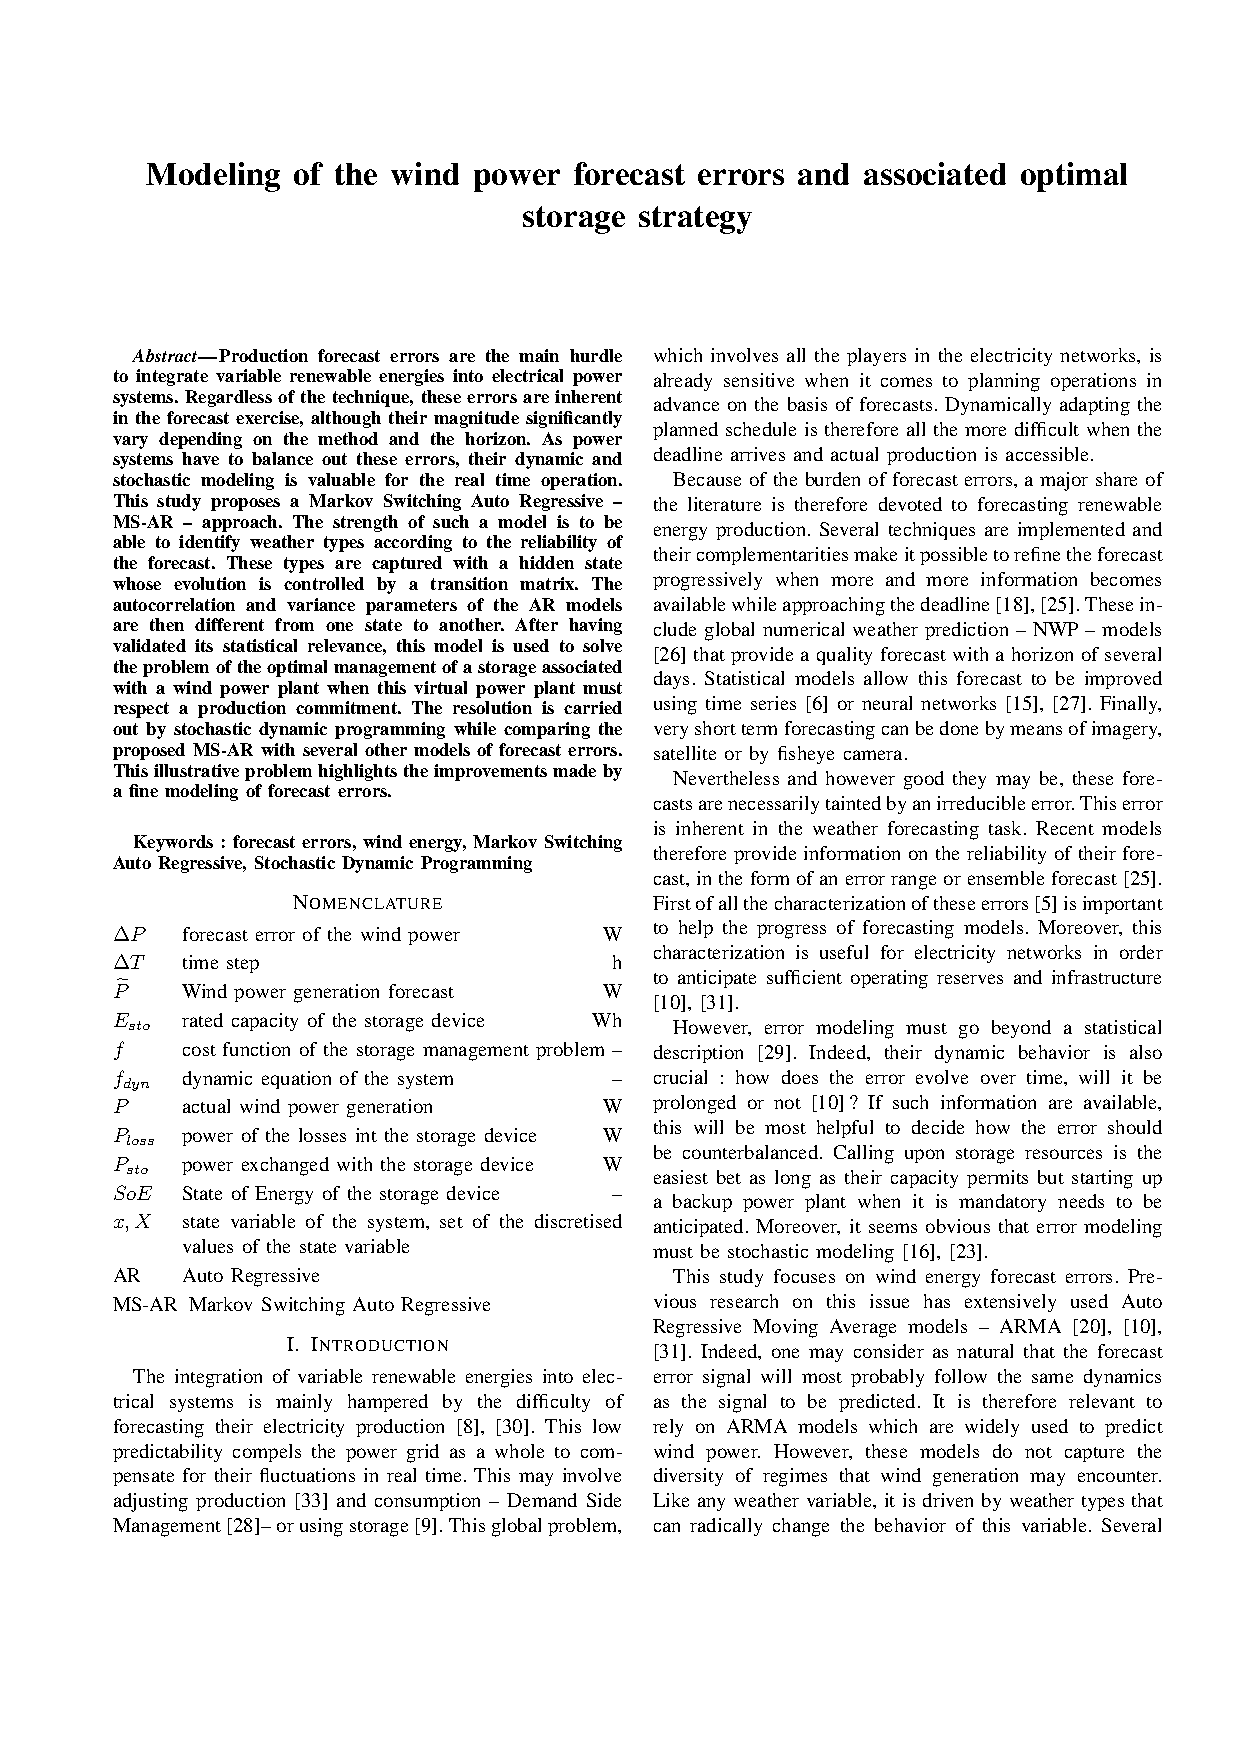
\includepdf[pages=-]{Images/Eolien/modeling-wind-power.pdf}


\bibliographystyle{IEEEtran}
\bibliography{Zotero}
\end{document}